\documentclass[twoside]{book}

% Packages required by doxygen
\usepackage{calc}
\usepackage{doxygen}
\usepackage{graphicx}
\usepackage[utf8]{inputenc}
\usepackage{makeidx}
\usepackage{multicol}
\usepackage{multirow}
\usepackage{textcomp}
\usepackage[table]{xcolor}

% Font selection
\usepackage[T1]{fontenc}
\usepackage{mathptmx}
\usepackage[scaled=.90]{helvet}
\usepackage{courier}
\usepackage{amssymb}
\usepackage{sectsty}
\renewcommand{\familydefault}{\sfdefault}
\allsectionsfont{%
  \fontseries{bc}\selectfont%
  \color{darkgray}%
}
\renewcommand{\DoxyLabelFont}{%
  \fontseries{bc}\selectfont%
  \color{darkgray}%
}

% Page & text layout
\usepackage{geometry}
\geometry{%
  a4paper,%
  top=2.5cm,%
  bottom=2.5cm,%
  left=2.5cm,%
  right=2.5cm%
}
\tolerance=750
\hfuzz=15pt
\hbadness=750
\setlength{\emergencystretch}{15pt}
\setlength{\parindent}{0cm}
\setlength{\parskip}{0.2cm}
\makeatletter
\renewcommand{\paragraph}{%
  \@startsection{paragraph}{4}{0ex}{-1.0ex}{1.0ex}{%
    \normalfont\normalsize\bfseries\SS@parafont%
  }%
}
\renewcommand{\subparagraph}{%
  \@startsection{subparagraph}{5}{0ex}{-1.0ex}{1.0ex}{%
    \normalfont\normalsize\bfseries\SS@subparafont%
  }%
}
\makeatother

% Headers & footers
\usepackage{fancyhdr}
\pagestyle{fancyplain}
\fancyhead[LE]{\fancyplain{}{\bfseries\thepage}}
\fancyhead[CE]{\fancyplain{}{}}
\fancyhead[RE]{\fancyplain{}{\bfseries\leftmark}}
\fancyhead[LO]{\fancyplain{}{\bfseries\rightmark}}
\fancyhead[CO]{\fancyplain{}{}}
\fancyhead[RO]{\fancyplain{}{\bfseries\thepage}}
\fancyfoot[LE]{\fancyplain{}{}}
\fancyfoot[CE]{\fancyplain{}{}}
\fancyfoot[RE]{\fancyplain{}{\bfseries\scriptsize Generated on Thu Nov 17 2016 14\-:01\-:19 for D\-P Václav Fanfule by Doxygen }}
\fancyfoot[LO]{\fancyplain{}{\bfseries\scriptsize Generated on Thu Nov 17 2016 14\-:01\-:19 for D\-P Václav Fanfule by Doxygen }}
\fancyfoot[CO]{\fancyplain{}{}}
\fancyfoot[RO]{\fancyplain{}{}}
\renewcommand{\footrulewidth}{0.4pt}
\renewcommand{\chaptermark}[1]{%
  \markboth{#1}{}%
}
\renewcommand{\sectionmark}[1]{%
  \markright{\thesection\ #1}%
}

% Indices & bibliography
\usepackage{natbib}
\usepackage[titles]{tocloft}
\setcounter{tocdepth}{3}
\setcounter{secnumdepth}{5}
\makeindex

% Hyperlinks (required, but should be loaded last)
\usepackage{ifpdf}
\ifpdf
  \usepackage[pdftex,pagebackref=true]{hyperref}
\else
  \usepackage[ps2pdf,pagebackref=true]{hyperref}
\fi
\hypersetup{%
  colorlinks=true,%
  linkcolor=blue,%
  citecolor=blue,%
  unicode%
}

% Custom commands
\newcommand{\clearemptydoublepage}{%
  \newpage{\pagestyle{empty}\cleardoublepage}%
}


%===== C O N T E N T S =====

\begin{document}

% Titlepage & ToC
\hypersetup{pageanchor=false}
\pagenumbering{roman}
\begin{titlepage}
\vspace*{7cm}
\begin{center}%
{\Large D\-P Václav Fanfule }\\
\vspace*{1cm}
{\large Generated by Doxygen 1.8.6}\\
\vspace*{0.5cm}
{\small Thu Nov 17 2016 14:01:19}\\
\end{center}
\end{titlepage}
\clearemptydoublepage
\tableofcontents
\clearemptydoublepage
\pagenumbering{arabic}
\hypersetup{pageanchor=true}

%--- Begin generated contents ---
\chapter{Class Index}
\section{Class List}
Here are the classes, structs, unions and interfaces with brief descriptions\-:\begin{DoxyCompactList}
\item\contentsline{section}{\hyperlink{structPictureData}{Picture\-Data} }{\pageref{structPictureData}}{}
\item\contentsline{section}{\hyperlink{structvector}{vector} }{\pageref{structvector}}{}
\end{DoxyCompactList}

\chapter{File Index}
\section{File List}
Here is a list of all files with brief descriptions\-:\begin{DoxyCompactList}
\item\contentsline{section}{src/\hyperlink{main_8cpp}{main.\-cpp} }{\pageref{main_8cpp}}{}
\item\contentsline{section}{src/\hyperlink{main_8h}{main.\-h} }{\pageref{main_8h}}{}
\item\contentsline{section}{src/\hyperlink{png__decode_8cpp}{png\-\_\-decode.\-cpp} }{\pageref{png__decode_8cpp}}{}
\item\contentsline{section}{src/\hyperlink{png__decode_8h}{png\-\_\-decode.\-h} }{\pageref{png__decode_8h}}{}
\item\contentsline{section}{src/\hyperlink{PSNR_8cpp}{P\-S\-N\-R.\-cpp} }{\pageref{PSNR_8cpp}}{}
\item\contentsline{section}{src/\hyperlink{psnr_8h}{psnr.\-h} }{\pageref{psnr_8h}}{}
\item\contentsline{section}{src/\hyperlink{SSIM_8cpp}{S\-S\-I\-M.\-cpp} }{\pageref{SSIM_8cpp}}{}
\item\contentsline{section}{src/\hyperlink{SSIM_8h}{S\-S\-I\-M.\-h} }{\pageref{SSIM_8h}}{}
\item\contentsline{section}{src/\hyperlink{stvssim_8cpp}{stvssim.\-cpp} }{\pageref{stvssim_8cpp}}{}
\item\contentsline{section}{src/\hyperlink{stvssim_8h}{stvssim.\-h} }{\pageref{stvssim_8h}}{}
\end{DoxyCompactList}

\chapter{Class Documentation}
\hypertarget{structPictureData}{\section{Picture\-Data Struct Reference}
\label{structPictureData}\index{Picture\-Data@{Picture\-Data}}
}


{\ttfamily \#include $<$main.\-h$>$}



Collaboration diagram for Picture\-Data\-:
\nopagebreak
\begin{figure}[H]
\begin{center}
\leavevmode
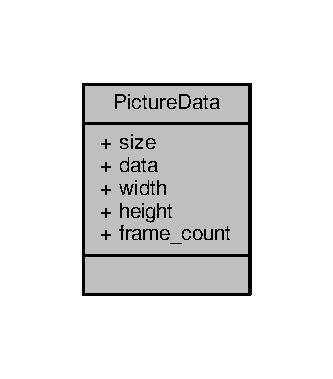
\includegraphics[width=160pt]{structPictureData__coll__graph}
\end{center}
\end{figure}
\subsection*{Public Attributes}
\begin{DoxyCompactItemize}
\item 
int \hyperlink{structPictureData_a2ca38938c35e5e26f27ea7089e8a394e}{size}
\item 
char $\ast$ \hyperlink{structPictureData_a2c18429fe90e5d541966cff885c56b16}{data}
\item 
int \hyperlink{structPictureData_a5bebf22e70c9d447b40a3bcf83906faa}{width}
\item 
int \hyperlink{structPictureData_ab0565ab5f2e7291c0b23982b1a25b2a7}{height}
\item 
int \hyperlink{structPictureData_a0ece02dd11b74f6ddd9e9d68132c4c70}{frame\-\_\-count}
\end{DoxyCompactItemize}


\subsection{Detailed Description}


Definition at line 1 of file main.\-h.



\subsection{Member Data Documentation}
\hypertarget{structPictureData_a2c18429fe90e5d541966cff885c56b16}{\index{Picture\-Data@{Picture\-Data}!data@{data}}
\index{data@{data}!PictureData@{Picture\-Data}}
\subsubsection[{data}]{\setlength{\rightskip}{0pt plus 5cm}char $\ast$ Picture\-Data\-::data}}\label{structPictureData_a2c18429fe90e5d541966cff885c56b16}


Definition at line 3 of file main.\-h.

\hypertarget{structPictureData_a0ece02dd11b74f6ddd9e9d68132c4c70}{\index{Picture\-Data@{Picture\-Data}!frame\-\_\-count@{frame\-\_\-count}}
\index{frame\-\_\-count@{frame\-\_\-count}!PictureData@{Picture\-Data}}
\subsubsection[{frame\-\_\-count}]{\setlength{\rightskip}{0pt plus 5cm}int Picture\-Data\-::frame\-\_\-count}}\label{structPictureData_a0ece02dd11b74f6ddd9e9d68132c4c70}


Definition at line 6 of file main.\-h.

\hypertarget{structPictureData_ab0565ab5f2e7291c0b23982b1a25b2a7}{\index{Picture\-Data@{Picture\-Data}!height@{height}}
\index{height@{height}!PictureData@{Picture\-Data}}
\subsubsection[{height}]{\setlength{\rightskip}{0pt plus 5cm}int Picture\-Data\-::height}}\label{structPictureData_ab0565ab5f2e7291c0b23982b1a25b2a7}


Definition at line 5 of file main.\-h.

\hypertarget{structPictureData_a2ca38938c35e5e26f27ea7089e8a394e}{\index{Picture\-Data@{Picture\-Data}!size@{size}}
\index{size@{size}!PictureData@{Picture\-Data}}
\subsubsection[{size}]{\setlength{\rightskip}{0pt plus 5cm}int Picture\-Data\-::size}}\label{structPictureData_a2ca38938c35e5e26f27ea7089e8a394e}


Definition at line 2 of file main.\-h.

\hypertarget{structPictureData_a5bebf22e70c9d447b40a3bcf83906faa}{\index{Picture\-Data@{Picture\-Data}!width@{width}}
\index{width@{width}!PictureData@{Picture\-Data}}
\subsubsection[{width}]{\setlength{\rightskip}{0pt plus 5cm}int Picture\-Data\-::width}}\label{structPictureData_a5bebf22e70c9d447b40a3bcf83906faa}


Definition at line 4 of file main.\-h.



The documentation for this struct was generated from the following files\-:\begin{DoxyCompactItemize}
\item 
src/\hyperlink{main_8h}{main.\-h}\item 
src/\hyperlink{png__decode_8h}{png\-\_\-decode.\-h}\end{DoxyCompactItemize}

\hypertarget{structvector}{\section{vector Struct Reference}
\label{structvector}\index{vector@{vector}}
}


{\ttfamily \#include $<$stvssim.\-h$>$}



Collaboration diagram for vector\-:
\nopagebreak
\begin{figure}[H]
\begin{center}
\leavevmode
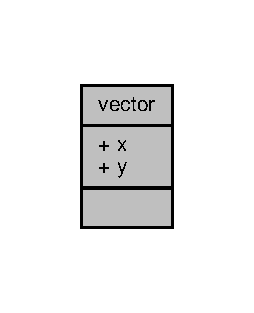
\includegraphics[width=122pt]{structvector__coll__graph}
\end{center}
\end{figure}
\subsection*{Public Attributes}
\begin{DoxyCompactItemize}
\item 
int \hyperlink{structvector_a0403eb3aea23a3009e276fba1d317046}{x}
\item 
int \hyperlink{structvector_aad6de640298eae97ca0a094db5aff477}{y}
\end{DoxyCompactItemize}


\subsection{Detailed Description}


Definition at line 15 of file stvssim.\-h.



\subsection{Member Data Documentation}
\hypertarget{structvector_a0403eb3aea23a3009e276fba1d317046}{\index{vector@{vector}!x@{x}}
\index{x@{x}!vector@{vector}}
\subsubsection[{x}]{\setlength{\rightskip}{0pt plus 5cm}int vector\-::x}}\label{structvector_a0403eb3aea23a3009e276fba1d317046}


Definition at line 16 of file stvssim.\-h.

\hypertarget{structvector_aad6de640298eae97ca0a094db5aff477}{\index{vector@{vector}!y@{y}}
\index{y@{y}!vector@{vector}}
\subsubsection[{y}]{\setlength{\rightskip}{0pt plus 5cm}int vector\-::y}}\label{structvector_aad6de640298eae97ca0a094db5aff477}


Definition at line 17 of file stvssim.\-h.



The documentation for this struct was generated from the following file\-:\begin{DoxyCompactItemize}
\item 
src/\hyperlink{stvssim_8h}{stvssim.\-h}\end{DoxyCompactItemize}

\chapter{File Documentation}
\hypertarget{main_8cpp}{\section{src/main.cpp File Reference}
\label{main_8cpp}\index{src/main.\-cpp@{src/main.\-cpp}}
}
{\ttfamily \#include $<$iostream$>$}\\*
{\ttfamily \#include $<$fstream$>$}\\*
{\ttfamily \#include $<$stdio.\-h$>$}\\*
{\ttfamily \#include $<$string.\-h$>$}\\*
{\ttfamily \#include $<$math.\-h$>$}\\*
{\ttfamily \#include $<$stdlib.\-h$>$}\\*
{\ttfamily \#include $<$cmath$>$}\\*
{\ttfamily \#include \char`\"{}S\-S\-I\-M.\-h\char`\"{}}\\*
{\ttfamily \#include \char`\"{}main.\-h\char`\"{}}\\*
{\ttfamily \#include \char`\"{}psnr.\-h\char`\"{}}\\*
{\ttfamily \#include \char`\"{}stvssim.\-h\char`\"{}}\\*
{\ttfamily \#include $<$omp.\-h$>$}\\*
Include dependency graph for main.\-cpp\-:
\nopagebreak
\begin{figure}[H]
\begin{center}
\leavevmode
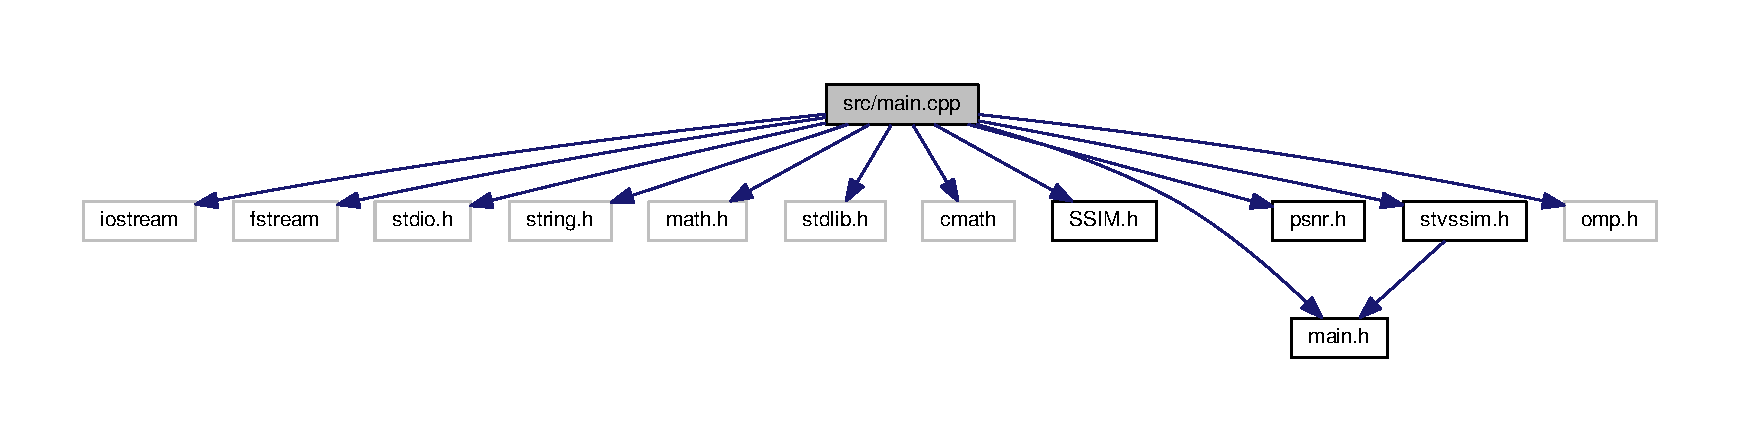
\includegraphics[width=350pt]{main_8cpp__incl}
\end{center}
\end{figure}
\subsection*{Macros}
\begin{DoxyCompactItemize}
\item 
\#define \hyperlink{main_8cpp_aea3cfda4f3a9f978ec759f206cf186fe}{C\-H\-U\-N\-K\-\_\-\-S\-I\-Z\-E}~1
\end{DoxyCompactItemize}
\subsection*{Functions}
\begin{DoxyCompactItemize}
\item 
int \hyperlink{main_8cpp_ac70138609ef6aa6fabca57aca8681e83}{compare} (const void $\ast$a, const void $\ast$b)
\item 
\hyperlink{structPictureData}{Picture\-Data} $\ast$ \hyperlink{main_8cpp_a65f6e83921f3a898f92c135c0853b37e}{get\-Video\-Info} (string path)
\item 
F\-I\-L\-E $\ast$ \hyperlink{main_8cpp_ada0df8f992e0e97e7ee6ae324a844273}{start\-F\-Fmpeg} (string path)
\item 
void \hyperlink{main_8cpp_a23d24ef0b8f8b2069dfe95630f8e9181}{shift\-Data} (unsigned char $\ast$$\ast$data, int size)
\item 
int \hyperlink{main_8cpp_a3c04138a5bfe5d72780bb7e82a18e627}{main} (int argc, char $\ast$$\ast$argv)
\end{DoxyCompactItemize}


\subsection{Macro Definition Documentation}
\hypertarget{main_8cpp_aea3cfda4f3a9f978ec759f206cf186fe}{\index{main.\-cpp@{main.\-cpp}!C\-H\-U\-N\-K\-\_\-\-S\-I\-Z\-E@{C\-H\-U\-N\-K\-\_\-\-S\-I\-Z\-E}}
\index{C\-H\-U\-N\-K\-\_\-\-S\-I\-Z\-E@{C\-H\-U\-N\-K\-\_\-\-S\-I\-Z\-E}!main.cpp@{main.\-cpp}}
\subsubsection[{C\-H\-U\-N\-K\-\_\-\-S\-I\-Z\-E}]{\setlength{\rightskip}{0pt plus 5cm}\#define C\-H\-U\-N\-K\-\_\-\-S\-I\-Z\-E~1}}\label{main_8cpp_aea3cfda4f3a9f978ec759f206cf186fe}


\subsection{Function Documentation}
\hypertarget{main_8cpp_ac70138609ef6aa6fabca57aca8681e83}{\index{main.\-cpp@{main.\-cpp}!compare@{compare}}
\index{compare@{compare}!main.cpp@{main.\-cpp}}
\subsubsection[{compare}]{\setlength{\rightskip}{0pt plus 5cm}int compare (
\begin{DoxyParamCaption}
\item[{const void $\ast$}]{a, }
\item[{const void $\ast$}]{b}
\end{DoxyParamCaption}
)}}\label{main_8cpp_ac70138609ef6aa6fabca57aca8681e83}


Definition at line 16 of file main.\-cpp.



Here is the caller graph for this function\-:
\nopagebreak
\begin{figure}[H]
\begin{center}
\leavevmode
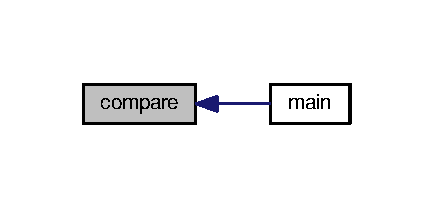
\includegraphics[width=208pt]{main_8cpp_ac70138609ef6aa6fabca57aca8681e83_icgraph}
\end{center}
\end{figure}


\hypertarget{main_8cpp_a65f6e83921f3a898f92c135c0853b37e}{\index{main.\-cpp@{main.\-cpp}!get\-Video\-Info@{get\-Video\-Info}}
\index{get\-Video\-Info@{get\-Video\-Info}!main.cpp@{main.\-cpp}}
\subsubsection[{get\-Video\-Info}]{\setlength{\rightskip}{0pt plus 5cm}{\bf Picture\-Data}$\ast$ get\-Video\-Info (
\begin{DoxyParamCaption}
\item[{string}]{path}
\end{DoxyParamCaption}
)}}\label{main_8cpp_a65f6e83921f3a898f92c135c0853b37e}


Definition at line 20 of file main.\-cpp.



Here is the caller graph for this function\-:
\nopagebreak
\begin{figure}[H]
\begin{center}
\leavevmode
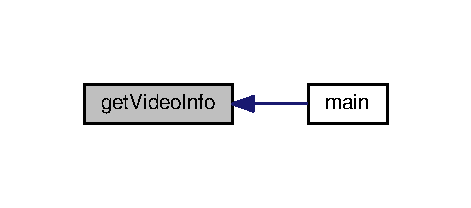
\includegraphics[width=226pt]{main_8cpp_a65f6e83921f3a898f92c135c0853b37e_icgraph}
\end{center}
\end{figure}


\hypertarget{main_8cpp_a3c04138a5bfe5d72780bb7e82a18e627}{\index{main.\-cpp@{main.\-cpp}!main@{main}}
\index{main@{main}!main.cpp@{main.\-cpp}}
\subsubsection[{main}]{\setlength{\rightskip}{0pt plus 5cm}int main (
\begin{DoxyParamCaption}
\item[{int}]{argc, }
\item[{char $\ast$$\ast$}]{argv}
\end{DoxyParamCaption}
)}}\label{main_8cpp_a3c04138a5bfe5d72780bb7e82a18e627}


Definition at line 81 of file main.\-cpp.



Here is the call graph for this function\-:
\nopagebreak
\begin{figure}[H]
\begin{center}
\leavevmode
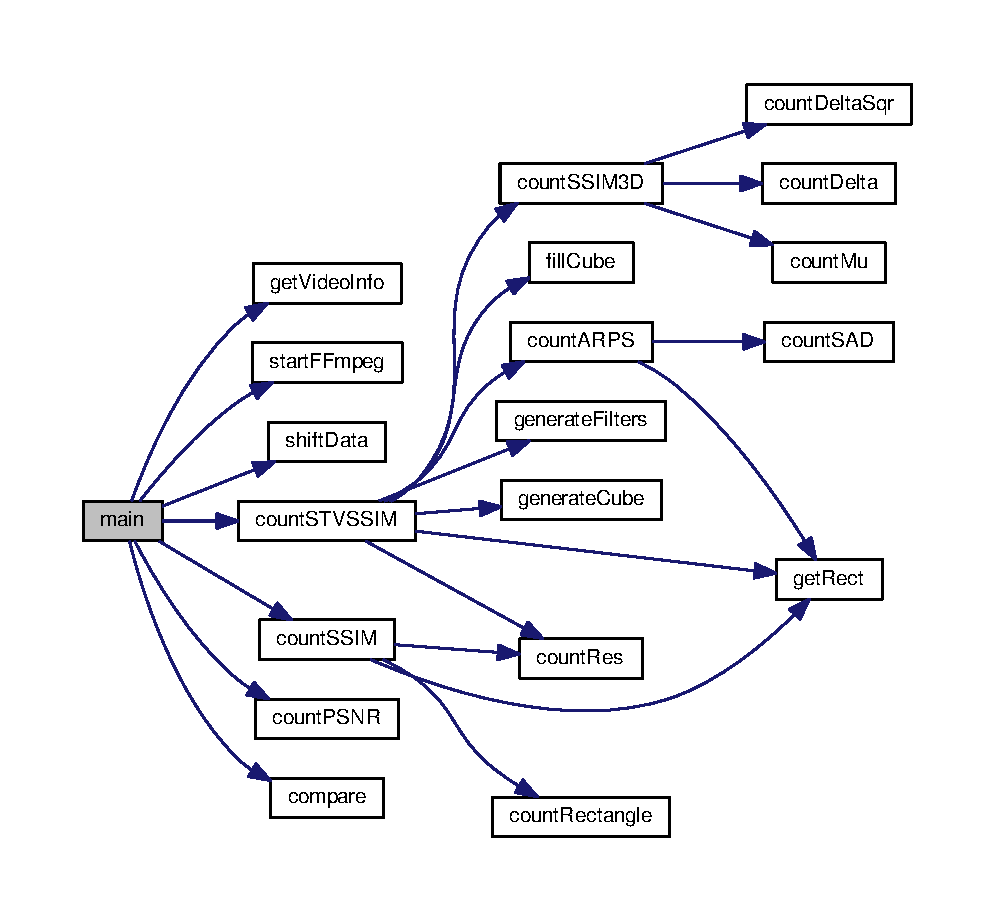
\includegraphics[width=350pt]{main_8cpp_a3c04138a5bfe5d72780bb7e82a18e627_cgraph}
\end{center}
\end{figure}


\hypertarget{main_8cpp_a23d24ef0b8f8b2069dfe95630f8e9181}{\index{main.\-cpp@{main.\-cpp}!shift\-Data@{shift\-Data}}
\index{shift\-Data@{shift\-Data}!main.cpp@{main.\-cpp}}
\subsubsection[{shift\-Data}]{\setlength{\rightskip}{0pt plus 5cm}void shift\-Data (
\begin{DoxyParamCaption}
\item[{unsigned char $\ast$$\ast$}]{data, }
\item[{int}]{size}
\end{DoxyParamCaption}
)}}\label{main_8cpp_a23d24ef0b8f8b2069dfe95630f8e9181}


Definition at line 73 of file main.\-cpp.



Here is the caller graph for this function\-:
\nopagebreak
\begin{figure}[H]
\begin{center}
\leavevmode
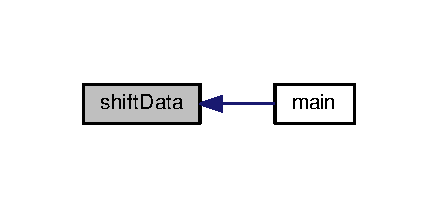
\includegraphics[width=210pt]{main_8cpp_a23d24ef0b8f8b2069dfe95630f8e9181_icgraph}
\end{center}
\end{figure}


\hypertarget{main_8cpp_ada0df8f992e0e97e7ee6ae324a844273}{\index{main.\-cpp@{main.\-cpp}!start\-F\-Fmpeg@{start\-F\-Fmpeg}}
\index{start\-F\-Fmpeg@{start\-F\-Fmpeg}!main.cpp@{main.\-cpp}}
\subsubsection[{start\-F\-Fmpeg}]{\setlength{\rightskip}{0pt plus 5cm}F\-I\-L\-E$\ast$ start\-F\-Fmpeg (
\begin{DoxyParamCaption}
\item[{string}]{path}
\end{DoxyParamCaption}
)}}\label{main_8cpp_ada0df8f992e0e97e7ee6ae324a844273}


Definition at line 56 of file main.\-cpp.



Here is the caller graph for this function\-:
\nopagebreak
\begin{figure}[H]
\begin{center}
\leavevmode
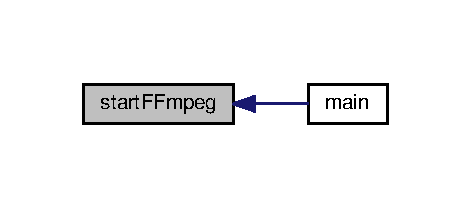
\includegraphics[width=226pt]{main_8cpp_ada0df8f992e0e97e7ee6ae324a844273_icgraph}
\end{center}
\end{figure}



\hypertarget{main_8h}{\section{src/main.h File Reference}
\label{main_8h}\index{src/main.\-h@{src/main.\-h}}
}
This graph shows which files directly or indirectly include this file\-:
\nopagebreak
\begin{figure}[H]
\begin{center}
\leavevmode
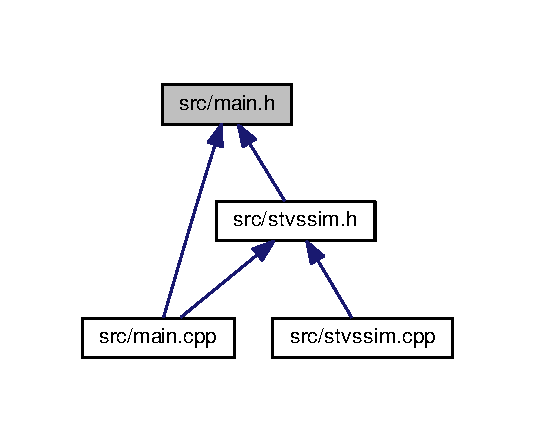
\includegraphics[width=257pt]{main_8h__dep__incl}
\end{center}
\end{figure}
\subsection*{Classes}
\begin{DoxyCompactItemize}
\item 
struct \hyperlink{structPictureData}{Picture\-Data}
\end{DoxyCompactItemize}
\subsection*{Macros}
\begin{DoxyCompactItemize}
\item 
\#define \hyperlink{main_8h_a2c5eecb22513a88c24ae5831a3265e54}{M\-A\-X\-\_\-\-F\-I\-L\-E\-S}~10
\item 
\#define \hyperlink{main_8h_a2fcfdf60d28725b11b5a3539d3acd0d4}{T\-H\-R\-E\-A\-D\-S}~256
\end{DoxyCompactItemize}


\subsection{Macro Definition Documentation}
\hypertarget{main_8h_a2c5eecb22513a88c24ae5831a3265e54}{\index{main.\-h@{main.\-h}!M\-A\-X\-\_\-\-F\-I\-L\-E\-S@{M\-A\-X\-\_\-\-F\-I\-L\-E\-S}}
\index{M\-A\-X\-\_\-\-F\-I\-L\-E\-S@{M\-A\-X\-\_\-\-F\-I\-L\-E\-S}!main.h@{main.\-h}}
\subsubsection[{M\-A\-X\-\_\-\-F\-I\-L\-E\-S}]{\setlength{\rightskip}{0pt plus 5cm}\#define M\-A\-X\-\_\-\-F\-I\-L\-E\-S~10}}\label{main_8h_a2c5eecb22513a88c24ae5831a3265e54}


Definition at line 10 of file main.\-h.

\hypertarget{main_8h_a2fcfdf60d28725b11b5a3539d3acd0d4}{\index{main.\-h@{main.\-h}!T\-H\-R\-E\-A\-D\-S@{T\-H\-R\-E\-A\-D\-S}}
\index{T\-H\-R\-E\-A\-D\-S@{T\-H\-R\-E\-A\-D\-S}!main.h@{main.\-h}}
\subsubsection[{T\-H\-R\-E\-A\-D\-S}]{\setlength{\rightskip}{0pt plus 5cm}\#define T\-H\-R\-E\-A\-D\-S~256}}\label{main_8h_a2fcfdf60d28725b11b5a3539d3acd0d4}


Definition at line 12 of file main.\-h.


\hypertarget{png__decode_8cpp}{\section{src/png\-\_\-decode.cpp File Reference}
\label{png__decode_8cpp}\index{src/png\-\_\-decode.\-cpp@{src/png\-\_\-decode.\-cpp}}
}
{\ttfamily \#include $<$stdlib.\-h$>$}\\*
{\ttfamily \#include $<$stdio.\-h$>$}\\*
{\ttfamily \#include $<$string.\-h$>$}\\*
{\ttfamily \#include $<$stdarg.\-h$>$}\\*
{\ttfamily \#include $<$iostream$>$}\\*
{\ttfamily \#include \char`\"{}png\-\_\-decode.\-h\char`\"{}}\\*
Include dependency graph for png\-\_\-decode.\-cpp\-:
\nopagebreak
\begin{figure}[H]
\begin{center}
\leavevmode
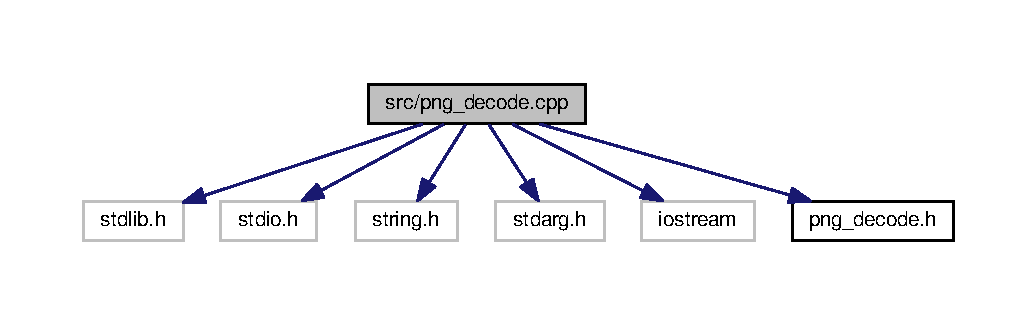
\includegraphics[width=350pt]{png__decode_8cpp__incl}
\end{center}
\end{figure}
\subsection*{Functions}
\begin{DoxyCompactItemize}
\item 
void \hyperlink{png__decode_8cpp_a7fe6a9c0c549657aa0d7da2e3c73fa01}{abort\-\_\-} (const char $\ast$s,...)
\item 
\hyperlink{structPictureData}{Picture\-Data} $\ast$ \hyperlink{png__decode_8cpp_ac47e45c677d42810fe262f4d9353912e}{read\-\_\-png\-\_\-file} (char $\ast$file\-\_\-name)
\item 
\hyperlink{structPictureData}{Picture\-Data} $\ast$ \hyperlink{png__decode_8cpp_a15766d3ba7e4f300d172280de6ef6a9e}{process\-\_\-file} (\hyperlink{structPictureData}{Picture\-Data} $\ast$data)
\end{DoxyCompactItemize}
\subsection*{Variables}
\begin{DoxyCompactItemize}
\item 
int \hyperlink{png__decode_8cpp_a6150e0515f7202e2fb518f7206ed97dc}{x}
\item 
int \hyperlink{png__decode_8cpp_a0a2f84ed7838f07779ae24c5a9086d33}{y}
\item 
int \hyperlink{png__decode_8cpp_add7425c568955bb79994730e77d38a18}{number\-\_\-of\-\_\-passes}
\end{DoxyCompactItemize}


\subsection{Function Documentation}
\hypertarget{png__decode_8cpp_a7fe6a9c0c549657aa0d7da2e3c73fa01}{\index{png\-\_\-decode.\-cpp@{png\-\_\-decode.\-cpp}!abort\-\_\-@{abort\-\_\-}}
\index{abort\-\_\-@{abort\-\_\-}!png_decode.cpp@{png\-\_\-decode.\-cpp}}
\subsubsection[{abort\-\_\-}]{\setlength{\rightskip}{0pt plus 5cm}void abort\-\_\- (
\begin{DoxyParamCaption}
\item[{const char $\ast$}]{s, }
\item[{}]{...}
\end{DoxyParamCaption}
)}}\label{png__decode_8cpp_a7fe6a9c0c549657aa0d7da2e3c73fa01}


Definition at line 11 of file png\-\_\-decode.\-cpp.



Here is the caller graph for this function\-:
\nopagebreak
\begin{figure}[H]
\begin{center}
\leavevmode
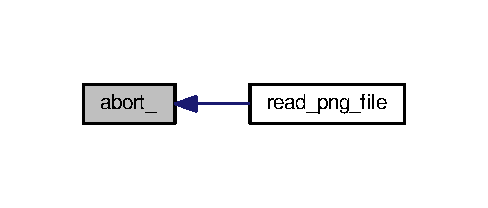
\includegraphics[width=234pt]{png__decode_8cpp_a7fe6a9c0c549657aa0d7da2e3c73fa01_icgraph}
\end{center}
\end{figure}


\hypertarget{png__decode_8cpp_a15766d3ba7e4f300d172280de6ef6a9e}{\index{png\-\_\-decode.\-cpp@{png\-\_\-decode.\-cpp}!process\-\_\-file@{process\-\_\-file}}
\index{process\-\_\-file@{process\-\_\-file}!png_decode.cpp@{png\-\_\-decode.\-cpp}}
\subsubsection[{process\-\_\-file}]{\setlength{\rightskip}{0pt plus 5cm}{\bf Picture\-Data}$\ast$ process\-\_\-file (
\begin{DoxyParamCaption}
\item[{{\bf Picture\-Data} $\ast$}]{data}
\end{DoxyParamCaption}
)}}\label{png__decode_8cpp_a15766d3ba7e4f300d172280de6ef6a9e}


Definition at line 84 of file png\-\_\-decode.\-cpp.



Here is the caller graph for this function\-:
\nopagebreak
\begin{figure}[H]
\begin{center}
\leavevmode
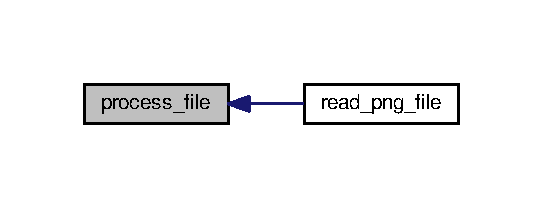
\includegraphics[width=260pt]{png__decode_8cpp_a15766d3ba7e4f300d172280de6ef6a9e_icgraph}
\end{center}
\end{figure}


\hypertarget{png__decode_8cpp_ac47e45c677d42810fe262f4d9353912e}{\index{png\-\_\-decode.\-cpp@{png\-\_\-decode.\-cpp}!read\-\_\-png\-\_\-file@{read\-\_\-png\-\_\-file}}
\index{read\-\_\-png\-\_\-file@{read\-\_\-png\-\_\-file}!png_decode.cpp@{png\-\_\-decode.\-cpp}}
\subsubsection[{read\-\_\-png\-\_\-file}]{\setlength{\rightskip}{0pt plus 5cm}{\bf Picture\-Data}$\ast$ read\-\_\-png\-\_\-file (
\begin{DoxyParamCaption}
\item[{char $\ast$}]{file\-\_\-name}
\end{DoxyParamCaption}
)}}\label{png__decode_8cpp_ac47e45c677d42810fe262f4d9353912e}


Definition at line 29 of file png\-\_\-decode.\-cpp.



Here is the call graph for this function\-:
\nopagebreak
\begin{figure}[H]
\begin{center}
\leavevmode
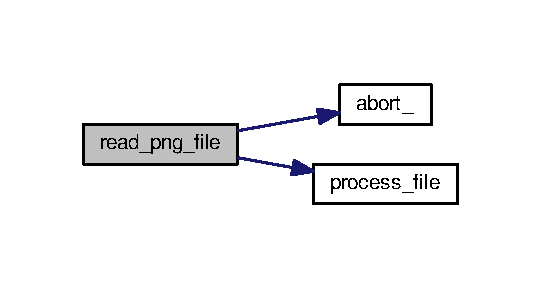
\includegraphics[width=260pt]{png__decode_8cpp_ac47e45c677d42810fe262f4d9353912e_cgraph}
\end{center}
\end{figure}




\subsection{Variable Documentation}
\hypertarget{png__decode_8cpp_add7425c568955bb79994730e77d38a18}{\index{png\-\_\-decode.\-cpp@{png\-\_\-decode.\-cpp}!number\-\_\-of\-\_\-passes@{number\-\_\-of\-\_\-passes}}
\index{number\-\_\-of\-\_\-passes@{number\-\_\-of\-\_\-passes}!png_decode.cpp@{png\-\_\-decode.\-cpp}}
\subsubsection[{number\-\_\-of\-\_\-passes}]{\setlength{\rightskip}{0pt plus 5cm}int number\-\_\-of\-\_\-passes}}\label{png__decode_8cpp_add7425c568955bb79994730e77d38a18}


Definition at line 24 of file png\-\_\-decode.\-cpp.

\hypertarget{png__decode_8cpp_a6150e0515f7202e2fb518f7206ed97dc}{\index{png\-\_\-decode.\-cpp@{png\-\_\-decode.\-cpp}!x@{x}}
\index{x@{x}!png_decode.cpp@{png\-\_\-decode.\-cpp}}
\subsubsection[{x}]{\setlength{\rightskip}{0pt plus 5cm}int x}}\label{png__decode_8cpp_a6150e0515f7202e2fb518f7206ed97dc}


Definition at line 21 of file png\-\_\-decode.\-cpp.

\hypertarget{png__decode_8cpp_a0a2f84ed7838f07779ae24c5a9086d33}{\index{png\-\_\-decode.\-cpp@{png\-\_\-decode.\-cpp}!y@{y}}
\index{y@{y}!png_decode.cpp@{png\-\_\-decode.\-cpp}}
\subsubsection[{y}]{\setlength{\rightskip}{0pt plus 5cm}int y}}\label{png__decode_8cpp_a0a2f84ed7838f07779ae24c5a9086d33}


Definition at line 21 of file png\-\_\-decode.\-cpp.


\hypertarget{png__decode_8h}{\section{src/png\-\_\-decode.h File Reference}
\label{png__decode_8h}\index{src/png\-\_\-decode.\-h@{src/png\-\_\-decode.\-h}}
}
This graph shows which files directly or indirectly include this file\-:
\nopagebreak
\begin{figure}[H]
\begin{center}
\leavevmode
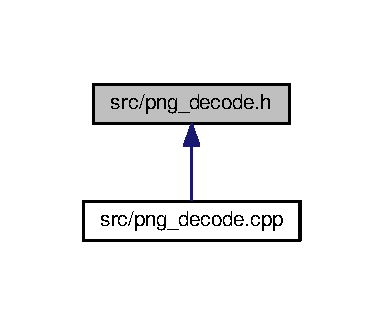
\includegraphics[width=184pt]{png__decode_8h__dep__incl}
\end{center}
\end{figure}
\subsection*{Classes}
\begin{DoxyCompactItemize}
\item 
struct \hyperlink{structPictureData}{Picture\-Data}
\end{DoxyCompactItemize}
\subsection*{Functions}
\begin{DoxyCompactItemize}
\item 
\hyperlink{structPictureData}{Picture\-Data} $\ast$ \hyperlink{png__decode_8h_a15766d3ba7e4f300d172280de6ef6a9e}{process\-\_\-file} (\hyperlink{structPictureData}{Picture\-Data} $\ast$data)
\item 
\hyperlink{structPictureData}{Picture\-Data} $\ast$ \hyperlink{png__decode_8h_ac47e45c677d42810fe262f4d9353912e}{read\-\_\-png\-\_\-file} (char $\ast$file\-\_\-name)
\end{DoxyCompactItemize}


\subsection{Function Documentation}
\hypertarget{png__decode_8h_a15766d3ba7e4f300d172280de6ef6a9e}{\index{png\-\_\-decode.\-h@{png\-\_\-decode.\-h}!process\-\_\-file@{process\-\_\-file}}
\index{process\-\_\-file@{process\-\_\-file}!png_decode.h@{png\-\_\-decode.\-h}}
\subsubsection[{process\-\_\-file}]{\setlength{\rightskip}{0pt plus 5cm}{\bf Picture\-Data}$\ast$ process\-\_\-file (
\begin{DoxyParamCaption}
\item[{{\bf Picture\-Data} $\ast$}]{data}
\end{DoxyParamCaption}
)}}\label{png__decode_8h_a15766d3ba7e4f300d172280de6ef6a9e}


Definition at line 84 of file png\-\_\-decode.\-cpp.



Here is the caller graph for this function\-:
\nopagebreak
\begin{figure}[H]
\begin{center}
\leavevmode
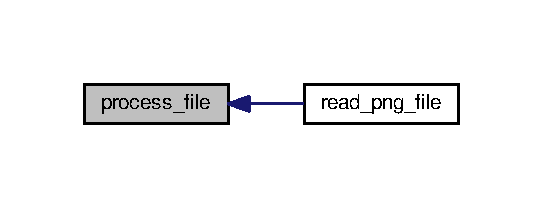
\includegraphics[width=260pt]{png__decode_8h_a15766d3ba7e4f300d172280de6ef6a9e_icgraph}
\end{center}
\end{figure}


\hypertarget{png__decode_8h_ac47e45c677d42810fe262f4d9353912e}{\index{png\-\_\-decode.\-h@{png\-\_\-decode.\-h}!read\-\_\-png\-\_\-file@{read\-\_\-png\-\_\-file}}
\index{read\-\_\-png\-\_\-file@{read\-\_\-png\-\_\-file}!png_decode.h@{png\-\_\-decode.\-h}}
\subsubsection[{read\-\_\-png\-\_\-file}]{\setlength{\rightskip}{0pt plus 5cm}{\bf Picture\-Data}$\ast$ read\-\_\-png\-\_\-file (
\begin{DoxyParamCaption}
\item[{char $\ast$}]{file\-\_\-name}
\end{DoxyParamCaption}
)}}\label{png__decode_8h_ac47e45c677d42810fe262f4d9353912e}


Definition at line 29 of file png\-\_\-decode.\-cpp.



Here is the call graph for this function\-:
\nopagebreak
\begin{figure}[H]
\begin{center}
\leavevmode
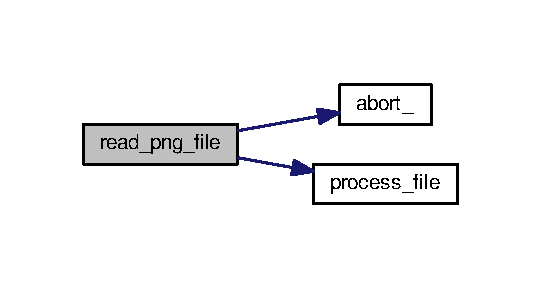
\includegraphics[width=260pt]{png__decode_8h_ac47e45c677d42810fe262f4d9353912e_cgraph}
\end{center}
\end{figure}



\hypertarget{PSNR_8cpp}{\section{src/\-P\-S\-N\-R.cpp File Reference}
\label{PSNR_8cpp}\index{src/\-P\-S\-N\-R.\-cpp@{src/\-P\-S\-N\-R.\-cpp}}
}
{\ttfamily \#include $<$iostream$>$}\\*
{\ttfamily \#include $<$fstream$>$}\\*
{\ttfamily \#include $<$stdio.\-h$>$}\\*
{\ttfamily \#include $<$string.\-h$>$}\\*
{\ttfamily \#include $<$math.\-h$>$}\\*
{\ttfamily \#include $<$stdlib.\-h$>$}\\*
{\ttfamily \#include $<$cmath$>$}\\*
{\ttfamily \#include \char`\"{}psnr.\-h\char`\"{}}\\*
{\ttfamily \#include $<$omp.\-h$>$}\\*
Include dependency graph for P\-S\-N\-R.\-cpp\-:
\nopagebreak
\begin{figure}[H]
\begin{center}
\leavevmode
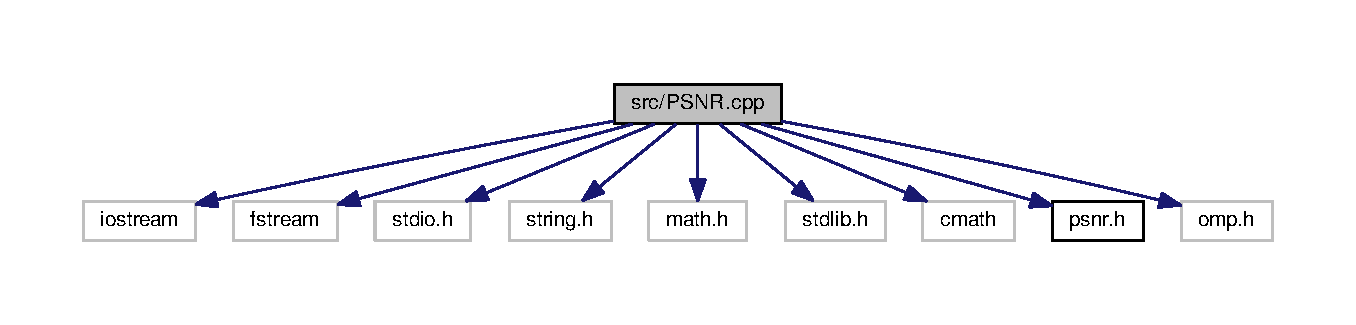
\includegraphics[width=350pt]{PSNR_8cpp__incl}
\end{center}
\end{figure}
\subsection*{Functions}
\begin{DoxyCompactItemize}
\item 
double \hyperlink{PSNR_8cpp_a40f074ee930b2b40b673a463bb0c089f}{count\-P\-S\-N\-R} (unsigned char $\ast$data1, unsigned char $\ast$data2, int size)
\end{DoxyCompactItemize}


\subsection{Function Documentation}
\hypertarget{PSNR_8cpp_a40f074ee930b2b40b673a463bb0c089f}{\index{P\-S\-N\-R.\-cpp@{P\-S\-N\-R.\-cpp}!count\-P\-S\-N\-R@{count\-P\-S\-N\-R}}
\index{count\-P\-S\-N\-R@{count\-P\-S\-N\-R}!PSNR.cpp@{P\-S\-N\-R.\-cpp}}
\subsubsection[{count\-P\-S\-N\-R}]{\setlength{\rightskip}{0pt plus 5cm}double count\-P\-S\-N\-R (
\begin{DoxyParamCaption}
\item[{unsigned char $\ast$}]{data1, }
\item[{unsigned char $\ast$}]{data2, }
\item[{int}]{size}
\end{DoxyParamCaption}
)}}\label{PSNR_8cpp_a40f074ee930b2b40b673a463bb0c089f}


Definition at line 22 of file P\-S\-N\-R.\-cpp.



Here is the caller graph for this function\-:
\nopagebreak
\begin{figure}[H]
\begin{center}
\leavevmode
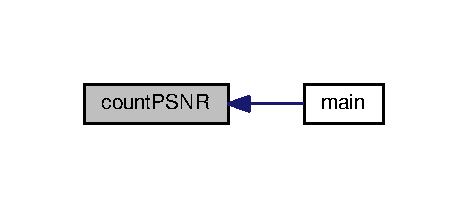
\includegraphics[width=224pt]{PSNR_8cpp_a40f074ee930b2b40b673a463bb0c089f_icgraph}
\end{center}
\end{figure}



\hypertarget{psnr_8h}{\section{src/psnr.h File Reference}
\label{psnr_8h}\index{src/psnr.\-h@{src/psnr.\-h}}
}
This graph shows which files directly or indirectly include this file\-:
\nopagebreak
\begin{figure}[H]
\begin{center}
\leavevmode
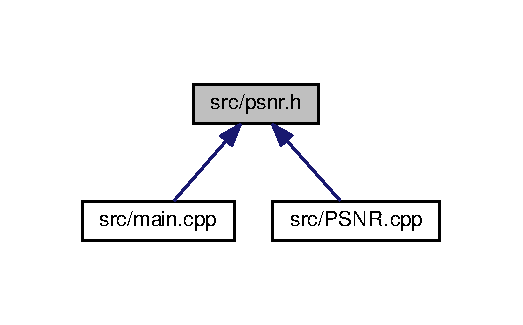
\includegraphics[width=251pt]{psnr_8h__dep__incl}
\end{center}
\end{figure}
\subsection*{Functions}
\begin{DoxyCompactItemize}
\item 
double \hyperlink{psnr_8h_a40f074ee930b2b40b673a463bb0c089f}{count\-P\-S\-N\-R} (unsigned char $\ast$data1, unsigned char $\ast$data2, int size)
\end{DoxyCompactItemize}


\subsection{Function Documentation}
\hypertarget{psnr_8h_a40f074ee930b2b40b673a463bb0c089f}{\index{psnr.\-h@{psnr.\-h}!count\-P\-S\-N\-R@{count\-P\-S\-N\-R}}
\index{count\-P\-S\-N\-R@{count\-P\-S\-N\-R}!psnr.h@{psnr.\-h}}
\subsubsection[{count\-P\-S\-N\-R}]{\setlength{\rightskip}{0pt plus 5cm}double count\-P\-S\-N\-R (
\begin{DoxyParamCaption}
\item[{unsigned char $\ast$}]{data1, }
\item[{unsigned char $\ast$}]{data2, }
\item[{int}]{size}
\end{DoxyParamCaption}
)}}\label{psnr_8h_a40f074ee930b2b40b673a463bb0c089f}


Definition at line 22 of file P\-S\-N\-R.\-cpp.



Here is the caller graph for this function\-:
\nopagebreak
\begin{figure}[H]
\begin{center}
\leavevmode
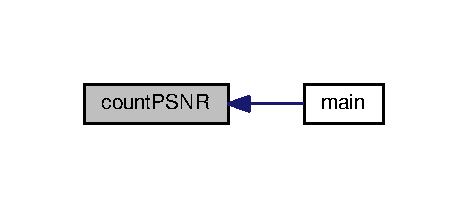
\includegraphics[width=224pt]{psnr_8h_a40f074ee930b2b40b673a463bb0c089f_icgraph}
\end{center}
\end{figure}



\hypertarget{SSIM_8cpp}{\section{src/\-S\-S\-I\-M.cpp File Reference}
\label{SSIM_8cpp}\index{src/\-S\-S\-I\-M.\-cpp@{src/\-S\-S\-I\-M.\-cpp}}
}
{\ttfamily \#include $<$iostream$>$}\\*
{\ttfamily \#include $<$fstream$>$}\\*
{\ttfamily \#include $<$stdio.\-h$>$}\\*
{\ttfamily \#include $<$string.\-h$>$}\\*
{\ttfamily \#include $<$math.\-h$>$}\\*
{\ttfamily \#include $<$stdlib.\-h$>$}\\*
{\ttfamily \#include $<$cmath$>$}\\*
{\ttfamily \#include \char`\"{}S\-S\-I\-M.\-h\char`\"{}}\\*
Include dependency graph for S\-S\-I\-M.\-cpp\-:
\nopagebreak
\begin{figure}[H]
\begin{center}
\leavevmode
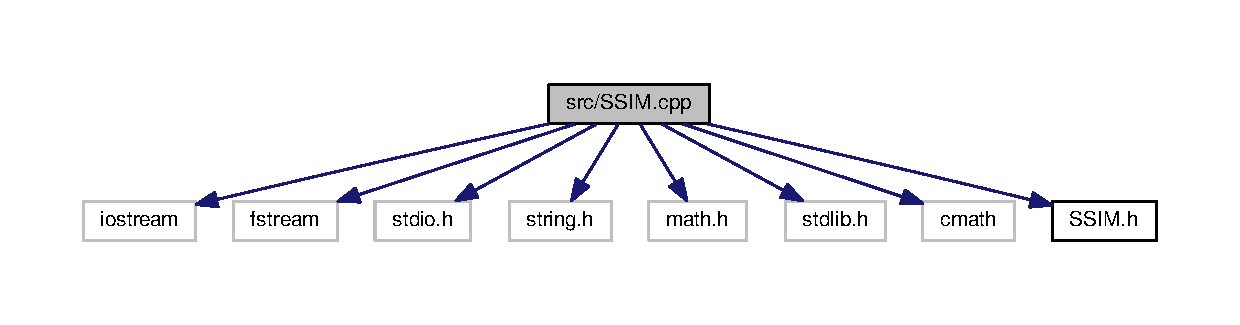
\includegraphics[width=350pt]{SSIM_8cpp__incl}
\end{center}
\end{figure}
\subsection*{Functions}
\begin{DoxyCompactItemize}
\item 
double \hyperlink{SSIM_8cpp_ae880e5b68d233da5e2a700216d45cd36}{count\-S\-S\-I\-M} (unsigned char $\ast$datain1, unsigned char $\ast$datain2, int size, int width)
\end{DoxyCompactItemize}


\subsection{Function Documentation}
\hypertarget{SSIM_8cpp_ae880e5b68d233da5e2a700216d45cd36}{\index{S\-S\-I\-M.\-cpp@{S\-S\-I\-M.\-cpp}!count\-S\-S\-I\-M@{count\-S\-S\-I\-M}}
\index{count\-S\-S\-I\-M@{count\-S\-S\-I\-M}!SSIM.cpp@{S\-S\-I\-M.\-cpp}}
\subsubsection[{count\-S\-S\-I\-M}]{\setlength{\rightskip}{0pt plus 5cm}double count\-S\-S\-I\-M (
\begin{DoxyParamCaption}
\item[{unsigned char $\ast$}]{datain1, }
\item[{unsigned char $\ast$}]{datain2, }
\item[{int}]{size, }
\item[{int}]{width}
\end{DoxyParamCaption}
)}}\label{SSIM_8cpp_ae880e5b68d233da5e2a700216d45cd36}


Definition at line 17 of file S\-S\-I\-M.\-cpp.



Here is the call graph for this function\-:
\nopagebreak
\begin{figure}[H]
\begin{center}
\leavevmode
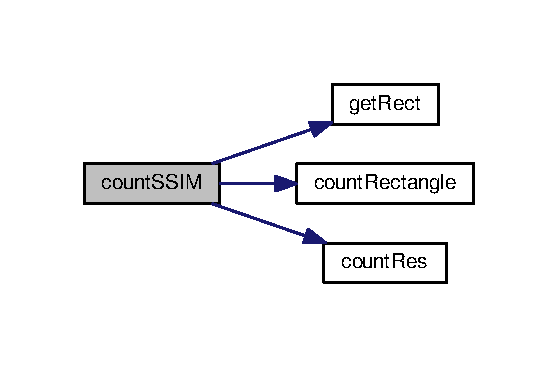
\includegraphics[width=268pt]{SSIM_8cpp_ae880e5b68d233da5e2a700216d45cd36_cgraph}
\end{center}
\end{figure}




Here is the caller graph for this function\-:
\nopagebreak
\begin{figure}[H]
\begin{center}
\leavevmode
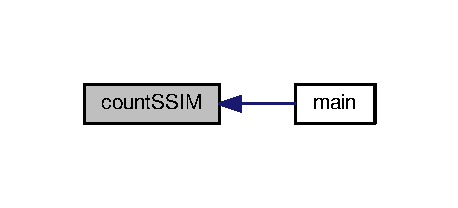
\includegraphics[width=220pt]{SSIM_8cpp_ae880e5b68d233da5e2a700216d45cd36_icgraph}
\end{center}
\end{figure}



\hypertarget{SSIM_8h}{\section{src/\-S\-S\-I\-M.h File Reference}
\label{SSIM_8h}\index{src/\-S\-S\-I\-M.\-h@{src/\-S\-S\-I\-M.\-h}}
}
This graph shows which files directly or indirectly include this file\-:
\nopagebreak
\begin{figure}[H]
\begin{center}
\leavevmode
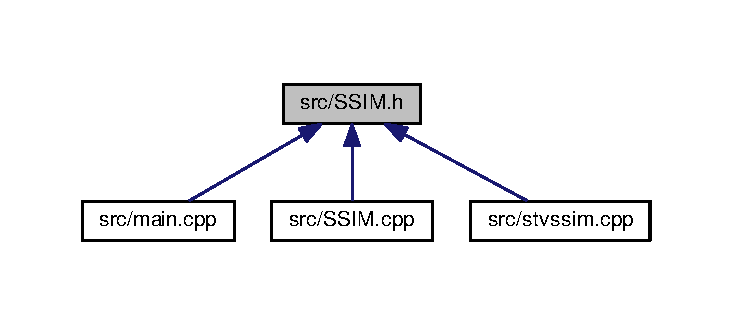
\includegraphics[width=350pt]{SSIM_8h__dep__incl}
\end{center}
\end{figure}
\subsection*{Macros}
\begin{DoxyCompactItemize}
\item 
\#define \hyperlink{SSIM_8h_ab60773f9d8d75ec04602ffb878732850}{R\-E\-C\-T\-\_\-\-S\-I\-Z\-E}~64
\item 
\#define \hyperlink{SSIM_8h_ac44b64f4a8ae9a6b66d304e070a17e41}{R\-E\-C\-T\-\_\-\-S\-Q\-R\-T}~8
\item 
\#define \hyperlink{SSIM_8h_a44779f18d87e71c78fc9fbf9dc88537d}{C1}~6.\-5025
\item 
\#define \hyperlink{SSIM_8h_ad6fc13322a4f1c314332ff34aa8b3fa0}{C2}~58.\-5225
\item 
\#define \hyperlink{SSIM_8h_a311ca79928cfdb061dc907246d321aed}{S\-K\-I\-P\-\_\-\-S\-I\-Z\-E}~8
\end{DoxyCompactItemize}
\subsection*{Functions}
\begin{DoxyCompactItemize}
\item 
double \hyperlink{SSIM_8h_ae880e5b68d233da5e2a700216d45cd36}{count\-S\-S\-I\-M} (unsigned char $\ast$datain1, unsigned char $\ast$datain2, int size, int width)
\item 
double \hyperlink{SSIM_8h_a63a05219d8b415024b4b5e02d1805786}{count\-Rectangle} (unsigned char $\ast$data1, unsigned char $\ast$data2)
\item 
double \hyperlink{SSIM_8h_a76ccde40000cac2ef79df0d64366f5a7}{count\-Avg} (unsigned char $\ast$data)
\item 
double \hyperlink{SSIM_8h_ab5437904deaec203620f72ef3b7fc862}{count\-Variance} (unsigned char $\ast$data, double avg)
\item 
double \hyperlink{SSIM_8h_a7c2b58cf78aabd67683c6acb3e2b45f6}{count\-Covariance} (unsigned char $\ast$data1, unsigned char $\ast$data2, double avg1, double avg2)
\item 
void \hyperlink{SSIM_8h_a3bd78652837ab363a2c8c7b6ebc71d17}{get\-Rect} (unsigned char $\ast$data, int start, int width, unsigned char $\ast$out)
\item 
double \hyperlink{SSIM_8h_ae29f8aaddab3087d2fb731a3a2f1f0eb}{count\-Res} (double $\ast$tmp\-Res, int count)
\end{DoxyCompactItemize}


\subsection{Macro Definition Documentation}
\hypertarget{SSIM_8h_a44779f18d87e71c78fc9fbf9dc88537d}{\index{S\-S\-I\-M.\-h@{S\-S\-I\-M.\-h}!C1@{C1}}
\index{C1@{C1}!SSIM.h@{S\-S\-I\-M.\-h}}
\subsubsection[{C1}]{\setlength{\rightskip}{0pt plus 5cm}\#define C1~6.\-5025}}\label{SSIM_8h_a44779f18d87e71c78fc9fbf9dc88537d}


Definition at line 12 of file S\-S\-I\-M.\-h.

\hypertarget{SSIM_8h_ad6fc13322a4f1c314332ff34aa8b3fa0}{\index{S\-S\-I\-M.\-h@{S\-S\-I\-M.\-h}!C2@{C2}}
\index{C2@{C2}!SSIM.h@{S\-S\-I\-M.\-h}}
\subsubsection[{C2}]{\setlength{\rightskip}{0pt plus 5cm}\#define C2~58.\-5225}}\label{SSIM_8h_ad6fc13322a4f1c314332ff34aa8b3fa0}


Definition at line 13 of file S\-S\-I\-M.\-h.

\hypertarget{SSIM_8h_ab60773f9d8d75ec04602ffb878732850}{\index{S\-S\-I\-M.\-h@{S\-S\-I\-M.\-h}!R\-E\-C\-T\-\_\-\-S\-I\-Z\-E@{R\-E\-C\-T\-\_\-\-S\-I\-Z\-E}}
\index{R\-E\-C\-T\-\_\-\-S\-I\-Z\-E@{R\-E\-C\-T\-\_\-\-S\-I\-Z\-E}!SSIM.h@{S\-S\-I\-M.\-h}}
\subsubsection[{R\-E\-C\-T\-\_\-\-S\-I\-Z\-E}]{\setlength{\rightskip}{0pt plus 5cm}\#define R\-E\-C\-T\-\_\-\-S\-I\-Z\-E~64}}\label{SSIM_8h_ab60773f9d8d75ec04602ffb878732850}


Definition at line 10 of file S\-S\-I\-M.\-h.

\hypertarget{SSIM_8h_ac44b64f4a8ae9a6b66d304e070a17e41}{\index{S\-S\-I\-M.\-h@{S\-S\-I\-M.\-h}!R\-E\-C\-T\-\_\-\-S\-Q\-R\-T@{R\-E\-C\-T\-\_\-\-S\-Q\-R\-T}}
\index{R\-E\-C\-T\-\_\-\-S\-Q\-R\-T@{R\-E\-C\-T\-\_\-\-S\-Q\-R\-T}!SSIM.h@{S\-S\-I\-M.\-h}}
\subsubsection[{R\-E\-C\-T\-\_\-\-S\-Q\-R\-T}]{\setlength{\rightskip}{0pt plus 5cm}\#define R\-E\-C\-T\-\_\-\-S\-Q\-R\-T~8}}\label{SSIM_8h_ac44b64f4a8ae9a6b66d304e070a17e41}


Definition at line 11 of file S\-S\-I\-M.\-h.

\hypertarget{SSIM_8h_a311ca79928cfdb061dc907246d321aed}{\index{S\-S\-I\-M.\-h@{S\-S\-I\-M.\-h}!S\-K\-I\-P\-\_\-\-S\-I\-Z\-E@{S\-K\-I\-P\-\_\-\-S\-I\-Z\-E}}
\index{S\-K\-I\-P\-\_\-\-S\-I\-Z\-E@{S\-K\-I\-P\-\_\-\-S\-I\-Z\-E}!SSIM.h@{S\-S\-I\-M.\-h}}
\subsubsection[{S\-K\-I\-P\-\_\-\-S\-I\-Z\-E}]{\setlength{\rightskip}{0pt plus 5cm}\#define S\-K\-I\-P\-\_\-\-S\-I\-Z\-E~8}}\label{SSIM_8h_a311ca79928cfdb061dc907246d321aed}


Definition at line 14 of file S\-S\-I\-M.\-h.



\subsection{Function Documentation}
\hypertarget{SSIM_8h_a76ccde40000cac2ef79df0d64366f5a7}{\index{S\-S\-I\-M.\-h@{S\-S\-I\-M.\-h}!count\-Avg@{count\-Avg}}
\index{count\-Avg@{count\-Avg}!SSIM.h@{S\-S\-I\-M.\-h}}
\subsubsection[{count\-Avg}]{\setlength{\rightskip}{0pt plus 5cm}double count\-Avg (
\begin{DoxyParamCaption}
\item[{unsigned char $\ast$}]{data}
\end{DoxyParamCaption}
)}}\label{SSIM_8h_a76ccde40000cac2ef79df0d64366f5a7}
\hypertarget{SSIM_8h_a7c2b58cf78aabd67683c6acb3e2b45f6}{\index{S\-S\-I\-M.\-h@{S\-S\-I\-M.\-h}!count\-Covariance@{count\-Covariance}}
\index{count\-Covariance@{count\-Covariance}!SSIM.h@{S\-S\-I\-M.\-h}}
\subsubsection[{count\-Covariance}]{\setlength{\rightskip}{0pt plus 5cm}double count\-Covariance (
\begin{DoxyParamCaption}
\item[{unsigned char $\ast$}]{data1, }
\item[{unsigned char $\ast$}]{data2, }
\item[{double}]{avg1, }
\item[{double}]{avg2}
\end{DoxyParamCaption}
)}}\label{SSIM_8h_a7c2b58cf78aabd67683c6acb3e2b45f6}
\hypertarget{SSIM_8h_a63a05219d8b415024b4b5e02d1805786}{\index{S\-S\-I\-M.\-h@{S\-S\-I\-M.\-h}!count\-Rectangle@{count\-Rectangle}}
\index{count\-Rectangle@{count\-Rectangle}!SSIM.h@{S\-S\-I\-M.\-h}}
\subsubsection[{count\-Rectangle}]{\setlength{\rightskip}{0pt plus 5cm}double count\-Rectangle (
\begin{DoxyParamCaption}
\item[{unsigned char $\ast$}]{data1, }
\item[{unsigned char $\ast$}]{data2}
\end{DoxyParamCaption}
)}}\label{SSIM_8h_a63a05219d8b415024b4b5e02d1805786}


Here is the caller graph for this function\-:
\nopagebreak
\begin{figure}[H]
\begin{center}
\leavevmode
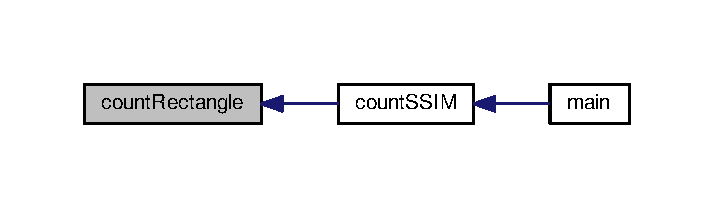
\includegraphics[width=342pt]{SSIM_8h_a63a05219d8b415024b4b5e02d1805786_icgraph}
\end{center}
\end{figure}


\hypertarget{SSIM_8h_ae29f8aaddab3087d2fb731a3a2f1f0eb}{\index{S\-S\-I\-M.\-h@{S\-S\-I\-M.\-h}!count\-Res@{count\-Res}}
\index{count\-Res@{count\-Res}!SSIM.h@{S\-S\-I\-M.\-h}}
\subsubsection[{count\-Res}]{\setlength{\rightskip}{0pt plus 5cm}double count\-Res (
\begin{DoxyParamCaption}
\item[{double $\ast$}]{tmp\-Res, }
\item[{int}]{count}
\end{DoxyParamCaption}
)}}\label{SSIM_8h_ae29f8aaddab3087d2fb731a3a2f1f0eb}


Here is the caller graph for this function\-:
\nopagebreak
\begin{figure}[H]
\begin{center}
\leavevmode
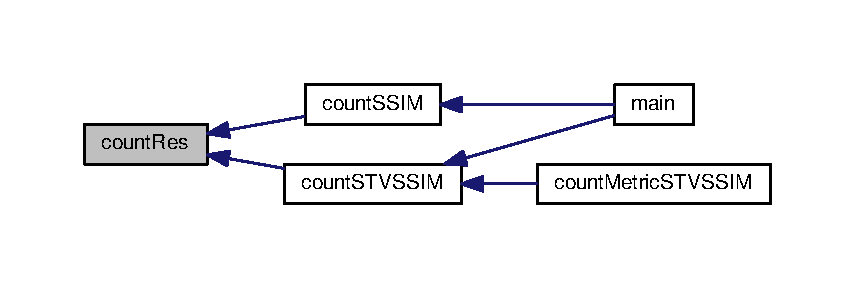
\includegraphics[width=350pt]{SSIM_8h_ae29f8aaddab3087d2fb731a3a2f1f0eb_icgraph}
\end{center}
\end{figure}


\hypertarget{SSIM_8h_ae880e5b68d233da5e2a700216d45cd36}{\index{S\-S\-I\-M.\-h@{S\-S\-I\-M.\-h}!count\-S\-S\-I\-M@{count\-S\-S\-I\-M}}
\index{count\-S\-S\-I\-M@{count\-S\-S\-I\-M}!SSIM.h@{S\-S\-I\-M.\-h}}
\subsubsection[{count\-S\-S\-I\-M}]{\setlength{\rightskip}{0pt plus 5cm}double count\-S\-S\-I\-M (
\begin{DoxyParamCaption}
\item[{unsigned char $\ast$}]{datain1, }
\item[{unsigned char $\ast$}]{datain2, }
\item[{int}]{size, }
\item[{int}]{width}
\end{DoxyParamCaption}
)}}\label{SSIM_8h_ae880e5b68d233da5e2a700216d45cd36}


Definition at line 17 of file S\-S\-I\-M.\-cpp.



Here is the call graph for this function\-:
\nopagebreak
\begin{figure}[H]
\begin{center}
\leavevmode
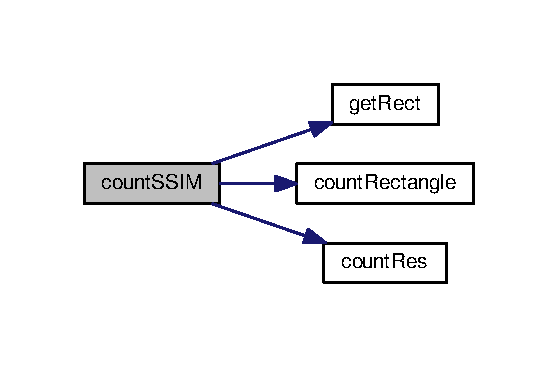
\includegraphics[width=268pt]{SSIM_8h_ae880e5b68d233da5e2a700216d45cd36_cgraph}
\end{center}
\end{figure}




Here is the caller graph for this function\-:
\nopagebreak
\begin{figure}[H]
\begin{center}
\leavevmode
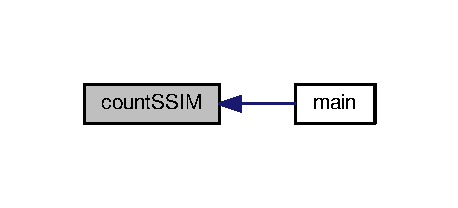
\includegraphics[width=220pt]{SSIM_8h_ae880e5b68d233da5e2a700216d45cd36_icgraph}
\end{center}
\end{figure}


\hypertarget{SSIM_8h_ab5437904deaec203620f72ef3b7fc862}{\index{S\-S\-I\-M.\-h@{S\-S\-I\-M.\-h}!count\-Variance@{count\-Variance}}
\index{count\-Variance@{count\-Variance}!SSIM.h@{S\-S\-I\-M.\-h}}
\subsubsection[{count\-Variance}]{\setlength{\rightskip}{0pt plus 5cm}double count\-Variance (
\begin{DoxyParamCaption}
\item[{unsigned char $\ast$}]{data, }
\item[{double}]{avg}
\end{DoxyParamCaption}
)}}\label{SSIM_8h_ab5437904deaec203620f72ef3b7fc862}
\hypertarget{SSIM_8h_a3bd78652837ab363a2c8c7b6ebc71d17}{\index{S\-S\-I\-M.\-h@{S\-S\-I\-M.\-h}!get\-Rect@{get\-Rect}}
\index{get\-Rect@{get\-Rect}!SSIM.h@{S\-S\-I\-M.\-h}}
\subsubsection[{get\-Rect}]{\setlength{\rightskip}{0pt plus 5cm}void get\-Rect (
\begin{DoxyParamCaption}
\item[{unsigned char $\ast$}]{data, }
\item[{int}]{start, }
\item[{int}]{width, }
\item[{unsigned char $\ast$}]{out}
\end{DoxyParamCaption}
)}}\label{SSIM_8h_a3bd78652837ab363a2c8c7b6ebc71d17}


Here is the caller graph for this function\-:
\nopagebreak
\begin{figure}[H]
\begin{center}
\leavevmode
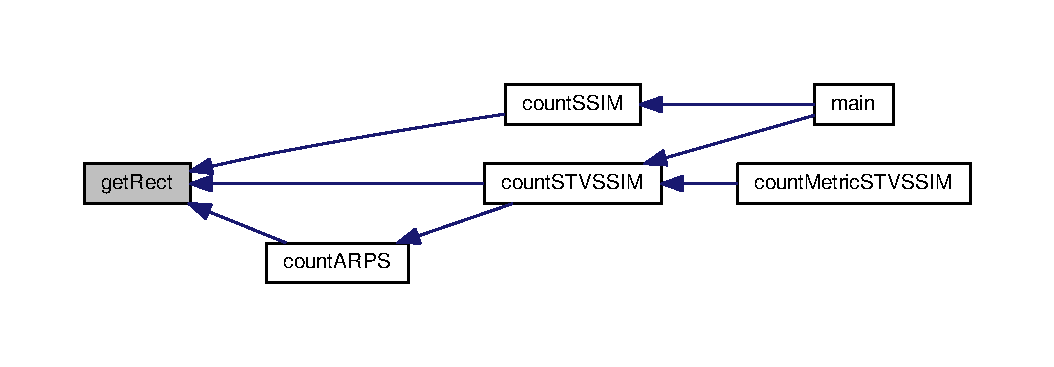
\includegraphics[width=350pt]{SSIM_8h_a3bd78652837ab363a2c8c7b6ebc71d17_icgraph}
\end{center}
\end{figure}



\hypertarget{stvssim_8cpp}{\section{src/stvssim.cpp File Reference}
\label{stvssim_8cpp}\index{src/stvssim.\-cpp@{src/stvssim.\-cpp}}
}
{\ttfamily \#include $<$iostream$>$}\\*
{\ttfamily \#include $<$fstream$>$}\\*
{\ttfamily \#include $<$stdio.\-h$>$}\\*
{\ttfamily \#include $<$string.\-h$>$}\\*
{\ttfamily \#include $<$math.\-h$>$}\\*
{\ttfamily \#include $<$stdlib.\-h$>$}\\*
{\ttfamily \#include $<$cmath$>$}\\*
{\ttfamily \#include \char`\"{}stvssim.\-h\char`\"{}}\\*
{\ttfamily \#include \char`\"{}S\-S\-I\-M.\-h\char`\"{}}\\*
{\ttfamily \#include $<$map$>$}\\*
Include dependency graph for stvssim.\-cpp\-:
\nopagebreak
\begin{figure}[H]
\begin{center}
\leavevmode
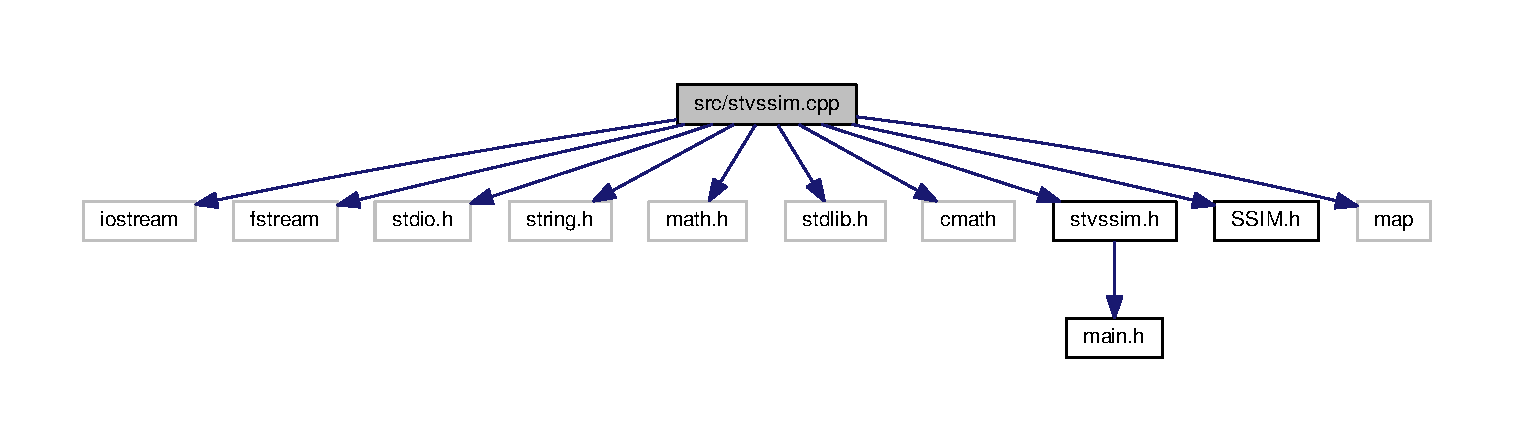
\includegraphics[width=350pt]{stvssim_8cpp__incl}
\end{center}
\end{figure}
\subsection*{Functions}
\begin{DoxyCompactItemize}
\item 
double $\ast$$\ast$ \hyperlink{stvssim_8cpp_ac69b5b2265122a1b7775640b8feb43e6}{count\-Metric\-S\-T\-V\-S\-S\-I\-M} (F\-I\-L\-E $\ast$$\ast$streams, F\-I\-L\-E $\ast$ref, int files\-\_\-count, \hyperlink{structPictureData}{Picture\-Data} $\ast$frame, string type, double $\ast$$\ast$results, int $\ast$\&frames)
\item 
double \hyperlink{stvssim_8cpp_aa188224c32927a5f4e14c264724276ca}{count\-S\-T\-V\-S\-S\-I\-M} (unsigned char $\ast$$\ast$datain1, unsigned char $\ast$$\ast$datain2, int size, int width)
\item 
double \hyperlink{stvssim_8cpp_ae40d916650014e6266ccbad2e3d08da9}{count\-S\-S\-I\-M3\-D} (unsigned char $\ast$$\ast$$\ast$filter, unsigned char $\ast$$\ast$$\ast$cube1, unsigned char $\ast$$\ast$$\ast$cube2)
\item 
double \hyperlink{stvssim_8cpp_ae81d1b26772887bce807b38ee044d8cf}{count\-Mu} (unsigned char $\ast$$\ast$$\ast$filter, unsigned char $\ast$$\ast$$\ast$cube)
\item 
double \hyperlink{stvssim_8cpp_a1afca8ffefb48e73d9749f0902e6770e}{count\-Delta\-Sqr} (unsigned char $\ast$$\ast$$\ast$filter, unsigned char $\ast$$\ast$$\ast$cube, double mu)
\item 
double \hyperlink{stvssim_8cpp_a32c2a80ad23848139ce03e3bf0d95b34}{count\-Delta} (unsigned char $\ast$$\ast$$\ast$filter, unsigned char $\ast$$\ast$$\ast$cube1, unsigned char $\ast$$\ast$$\ast$cube2, double mu\-X, double mu\-Y)
\item 
unsigned char $\ast$$\ast$$\ast$ \hyperlink{stvssim_8cpp_aee5cce2c1f90ed16082c6f01eb8eb2ed}{generate\-Cube} ()
\item 
void \hyperlink{stvssim_8cpp_acafb1bf84ccd5750b7745d814c792560}{fill\-Cube} (unsigned char $\ast$$\ast$datain, int pos, unsigned char $\ast$$\ast$$\ast$out, int width)
\item 
unsigned char $\ast$$\ast$$\ast$$\ast$ \hyperlink{stvssim_8cpp_a4094691210615420943d90d66fed89f0}{generate\-Filters} ()
\item 
\hyperlink{structvector}{vector} \hyperlink{stvssim_8cpp_a6aeaebf5f578aac2e9bdbf3151a571c5}{count\-A\-R\-P\-S} (unsigned char $\ast$block, unsigned char $\ast$frame\-Prev, int \hyperlink{png__decode_8cpp_a6150e0515f7202e2fb518f7206ed97dc}{x}, int \hyperlink{png__decode_8cpp_a0a2f84ed7838f07779ae24c5a9086d33}{y}, int width, int height, int T)
\item 
void \hyperlink{stvssim_8cpp_a23d24ef0b8f8b2069dfe95630f8e9181}{shift\-Data} (unsigned char $\ast$$\ast$data, int size)
\item 
int \hyperlink{stvssim_8cpp_a0b34f8c2a0ca35e66931ea883c66397e}{count\-S\-A\-D} (unsigned char $\ast$rect1, unsigned char $\ast$rect2)
\end{DoxyCompactItemize}


\subsection{Function Documentation}
\hypertarget{stvssim_8cpp_a6aeaebf5f578aac2e9bdbf3151a571c5}{\index{stvssim.\-cpp@{stvssim.\-cpp}!count\-A\-R\-P\-S@{count\-A\-R\-P\-S}}
\index{count\-A\-R\-P\-S@{count\-A\-R\-P\-S}!stvssim.cpp@{stvssim.\-cpp}}
\subsubsection[{count\-A\-R\-P\-S}]{\setlength{\rightskip}{0pt plus 5cm}{\bf vector} count\-A\-R\-P\-S (
\begin{DoxyParamCaption}
\item[{unsigned char $\ast$}]{block, }
\item[{unsigned char $\ast$}]{frame\-Prev, }
\item[{int}]{x, }
\item[{int}]{y, }
\item[{int}]{width, }
\item[{int}]{height, }
\item[{int}]{T}
\end{DoxyParamCaption}
)}}\label{stvssim_8cpp_a6aeaebf5f578aac2e9bdbf3151a571c5}


Definition at line 316 of file stvssim.\-cpp.



Here is the call graph for this function\-:
\nopagebreak
\begin{figure}[H]
\begin{center}
\leavevmode
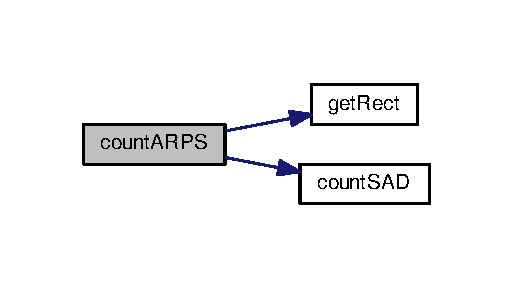
\includegraphics[width=246pt]{stvssim_8cpp_a6aeaebf5f578aac2e9bdbf3151a571c5_cgraph}
\end{center}
\end{figure}




Here is the caller graph for this function\-:
\nopagebreak
\begin{figure}[H]
\begin{center}
\leavevmode
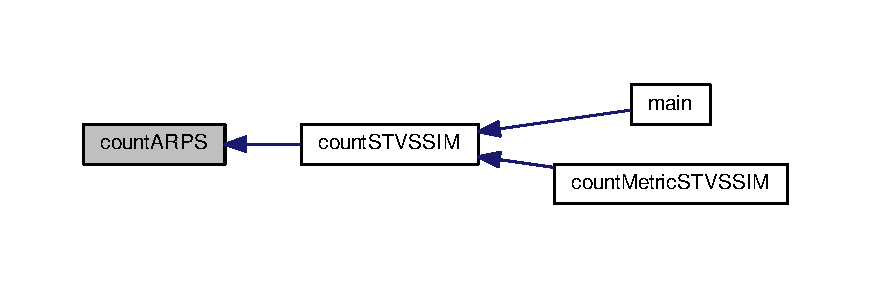
\includegraphics[width=350pt]{stvssim_8cpp_a6aeaebf5f578aac2e9bdbf3151a571c5_icgraph}
\end{center}
\end{figure}


\hypertarget{stvssim_8cpp_a32c2a80ad23848139ce03e3bf0d95b34}{\index{stvssim.\-cpp@{stvssim.\-cpp}!count\-Delta@{count\-Delta}}
\index{count\-Delta@{count\-Delta}!stvssim.cpp@{stvssim.\-cpp}}
\subsubsection[{count\-Delta}]{\setlength{\rightskip}{0pt plus 5cm}double count\-Delta (
\begin{DoxyParamCaption}
\item[{unsigned char $\ast$$\ast$$\ast$}]{filter, }
\item[{unsigned char $\ast$$\ast$$\ast$}]{cube1, }
\item[{unsigned char $\ast$$\ast$$\ast$}]{cube2, }
\item[{double}]{mu\-X, }
\item[{double}]{mu\-Y}
\end{DoxyParamCaption}
)}}\label{stvssim_8cpp_a32c2a80ad23848139ce03e3bf0d95b34}


Definition at line 235 of file stvssim.\-cpp.



Here is the caller graph for this function\-:
\nopagebreak
\begin{figure}[H]
\begin{center}
\leavevmode
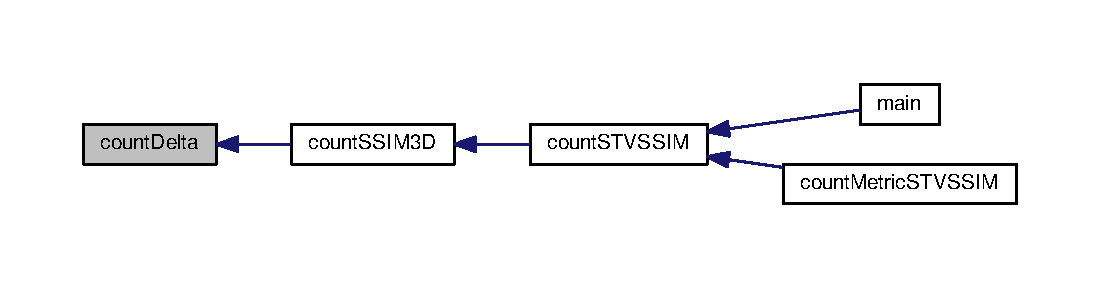
\includegraphics[width=350pt]{stvssim_8cpp_a32c2a80ad23848139ce03e3bf0d95b34_icgraph}
\end{center}
\end{figure}


\hypertarget{stvssim_8cpp_a1afca8ffefb48e73d9749f0902e6770e}{\index{stvssim.\-cpp@{stvssim.\-cpp}!count\-Delta\-Sqr@{count\-Delta\-Sqr}}
\index{count\-Delta\-Sqr@{count\-Delta\-Sqr}!stvssim.cpp@{stvssim.\-cpp}}
\subsubsection[{count\-Delta\-Sqr}]{\setlength{\rightskip}{0pt plus 5cm}double count\-Delta\-Sqr (
\begin{DoxyParamCaption}
\item[{unsigned char $\ast$$\ast$$\ast$}]{filter, }
\item[{unsigned char $\ast$$\ast$$\ast$}]{cube, }
\item[{double}]{mu}
\end{DoxyParamCaption}
)}}\label{stvssim_8cpp_a1afca8ffefb48e73d9749f0902e6770e}


Definition at line 222 of file stvssim.\-cpp.



Here is the caller graph for this function\-:
\nopagebreak
\begin{figure}[H]
\begin{center}
\leavevmode
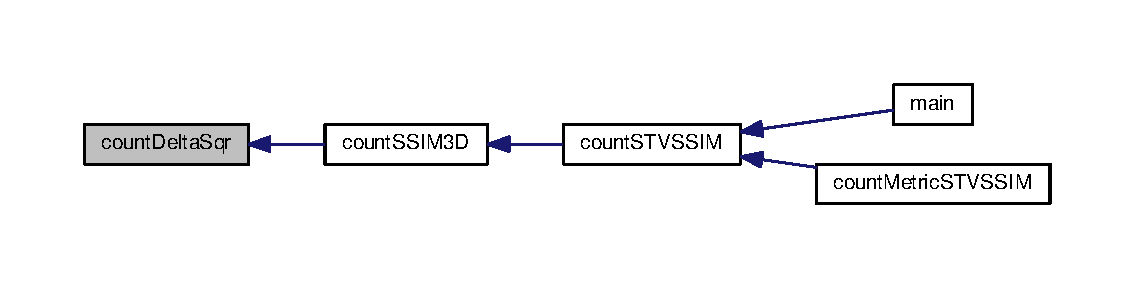
\includegraphics[width=350pt]{stvssim_8cpp_a1afca8ffefb48e73d9749f0902e6770e_icgraph}
\end{center}
\end{figure}


\hypertarget{stvssim_8cpp_ac69b5b2265122a1b7775640b8feb43e6}{\index{stvssim.\-cpp@{stvssim.\-cpp}!count\-Metric\-S\-T\-V\-S\-S\-I\-M@{count\-Metric\-S\-T\-V\-S\-S\-I\-M}}
\index{count\-Metric\-S\-T\-V\-S\-S\-I\-M@{count\-Metric\-S\-T\-V\-S\-S\-I\-M}!stvssim.cpp@{stvssim.\-cpp}}
\subsubsection[{count\-Metric\-S\-T\-V\-S\-S\-I\-M}]{\setlength{\rightskip}{0pt plus 5cm}double$\ast$$\ast$ count\-Metric\-S\-T\-V\-S\-S\-I\-M (
\begin{DoxyParamCaption}
\item[{F\-I\-L\-E $\ast$$\ast$}]{streams, }
\item[{F\-I\-L\-E $\ast$}]{ref, }
\item[{int}]{files\-\_\-count, }
\item[{{\bf Picture\-Data} $\ast$}]{frame, }
\item[{string}]{type, }
\item[{double $\ast$$\ast$}]{results, }
\item[{int $\ast$\&}]{frames}
\end{DoxyParamCaption}
)}}\label{stvssim_8cpp_ac69b5b2265122a1b7775640b8feb43e6}


Definition at line 16 of file stvssim.\-cpp.



Here is the call graph for this function\-:
\nopagebreak
\begin{figure}[H]
\begin{center}
\leavevmode
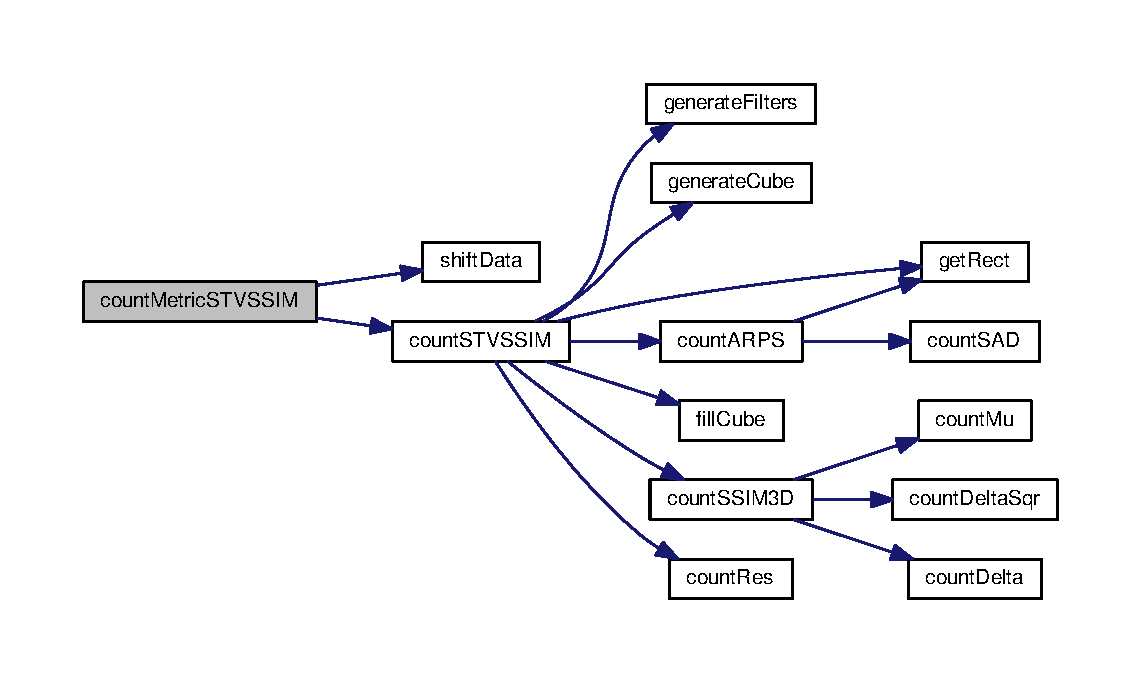
\includegraphics[width=350pt]{stvssim_8cpp_ac69b5b2265122a1b7775640b8feb43e6_cgraph}
\end{center}
\end{figure}


\hypertarget{stvssim_8cpp_ae81d1b26772887bce807b38ee044d8cf}{\index{stvssim.\-cpp@{stvssim.\-cpp}!count\-Mu@{count\-Mu}}
\index{count\-Mu@{count\-Mu}!stvssim.cpp@{stvssim.\-cpp}}
\subsubsection[{count\-Mu}]{\setlength{\rightskip}{0pt plus 5cm}double count\-Mu (
\begin{DoxyParamCaption}
\item[{unsigned char $\ast$$\ast$$\ast$}]{filter, }
\item[{unsigned char $\ast$$\ast$$\ast$}]{cube}
\end{DoxyParamCaption}
)}}\label{stvssim_8cpp_ae81d1b26772887bce807b38ee044d8cf}


Definition at line 208 of file stvssim.\-cpp.



Here is the caller graph for this function\-:
\nopagebreak
\begin{figure}[H]
\begin{center}
\leavevmode
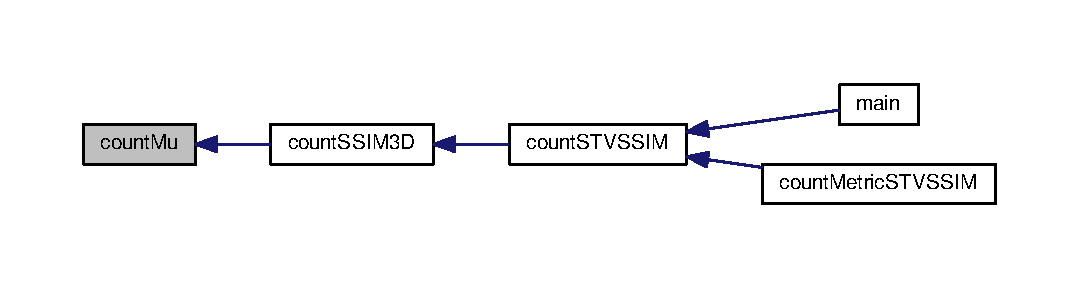
\includegraphics[width=350pt]{stvssim_8cpp_ae81d1b26772887bce807b38ee044d8cf_icgraph}
\end{center}
\end{figure}


\hypertarget{stvssim_8cpp_a0b34f8c2a0ca35e66931ea883c66397e}{\index{stvssim.\-cpp@{stvssim.\-cpp}!count\-S\-A\-D@{count\-S\-A\-D}}
\index{count\-S\-A\-D@{count\-S\-A\-D}!stvssim.cpp@{stvssim.\-cpp}}
\subsubsection[{count\-S\-A\-D}]{\setlength{\rightskip}{0pt plus 5cm}int count\-S\-A\-D (
\begin{DoxyParamCaption}
\item[{unsigned char $\ast$}]{rect1, }
\item[{unsigned char $\ast$}]{rect2}
\end{DoxyParamCaption}
)}}\label{stvssim_8cpp_a0b34f8c2a0ca35e66931ea883c66397e}


Definition at line 390 of file stvssim.\-cpp.



Here is the caller graph for this function\-:
\nopagebreak
\begin{figure}[H]
\begin{center}
\leavevmode
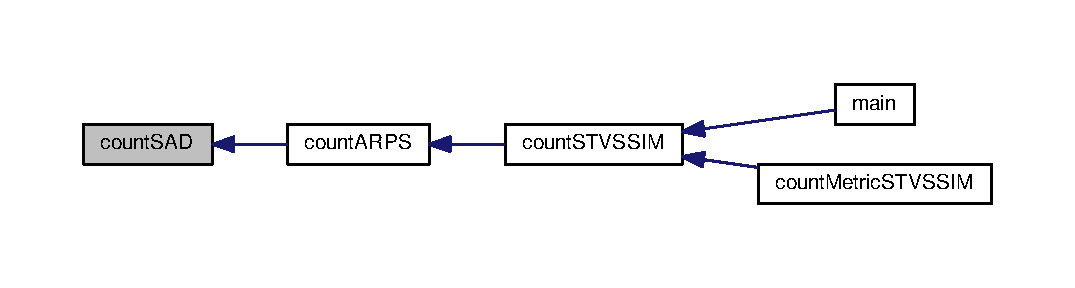
\includegraphics[width=350pt]{stvssim_8cpp_a0b34f8c2a0ca35e66931ea883c66397e_icgraph}
\end{center}
\end{figure}


\hypertarget{stvssim_8cpp_ae40d916650014e6266ccbad2e3d08da9}{\index{stvssim.\-cpp@{stvssim.\-cpp}!count\-S\-S\-I\-M3\-D@{count\-S\-S\-I\-M3\-D}}
\index{count\-S\-S\-I\-M3\-D@{count\-S\-S\-I\-M3\-D}!stvssim.cpp@{stvssim.\-cpp}}
\subsubsection[{count\-S\-S\-I\-M3\-D}]{\setlength{\rightskip}{0pt plus 5cm}double count\-S\-S\-I\-M3\-D (
\begin{DoxyParamCaption}
\item[{unsigned char $\ast$$\ast$$\ast$}]{filter, }
\item[{unsigned char $\ast$$\ast$$\ast$}]{cube1, }
\item[{unsigned char $\ast$$\ast$$\ast$}]{cube2}
\end{DoxyParamCaption}
)}}\label{stvssim_8cpp_ae40d916650014e6266ccbad2e3d08da9}


Definition at line 196 of file stvssim.\-cpp.



Here is the call graph for this function\-:
\nopagebreak
\begin{figure}[H]
\begin{center}
\leavevmode
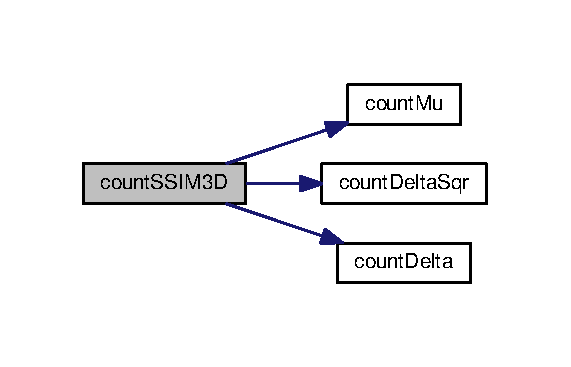
\includegraphics[width=274pt]{stvssim_8cpp_ae40d916650014e6266ccbad2e3d08da9_cgraph}
\end{center}
\end{figure}




Here is the caller graph for this function\-:
\nopagebreak
\begin{figure}[H]
\begin{center}
\leavevmode
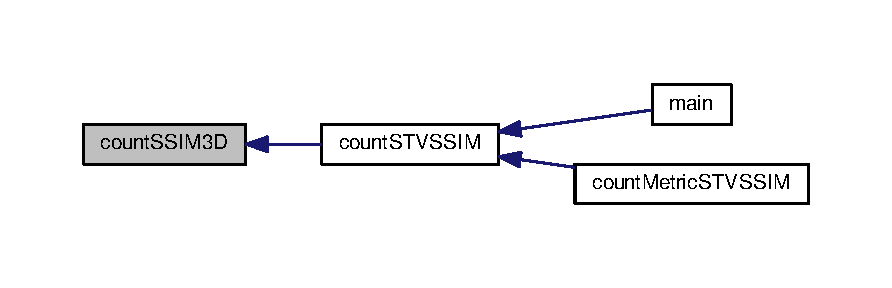
\includegraphics[width=350pt]{stvssim_8cpp_ae40d916650014e6266ccbad2e3d08da9_icgraph}
\end{center}
\end{figure}


\hypertarget{stvssim_8cpp_aa188224c32927a5f4e14c264724276ca}{\index{stvssim.\-cpp@{stvssim.\-cpp}!count\-S\-T\-V\-S\-S\-I\-M@{count\-S\-T\-V\-S\-S\-I\-M}}
\index{count\-S\-T\-V\-S\-S\-I\-M@{count\-S\-T\-V\-S\-S\-I\-M}!stvssim.cpp@{stvssim.\-cpp}}
\subsubsection[{count\-S\-T\-V\-S\-S\-I\-M}]{\setlength{\rightskip}{0pt plus 5cm}double count\-S\-T\-V\-S\-S\-I\-M (
\begin{DoxyParamCaption}
\item[{unsigned char $\ast$$\ast$}]{datain1, }
\item[{unsigned char $\ast$$\ast$}]{datain2, }
\item[{int}]{size, }
\item[{int}]{width}
\end{DoxyParamCaption}
)}}\label{stvssim_8cpp_aa188224c32927a5f4e14c264724276ca}


Definition at line 81 of file stvssim.\-cpp.



Here is the call graph for this function\-:
\nopagebreak
\begin{figure}[H]
\begin{center}
\leavevmode
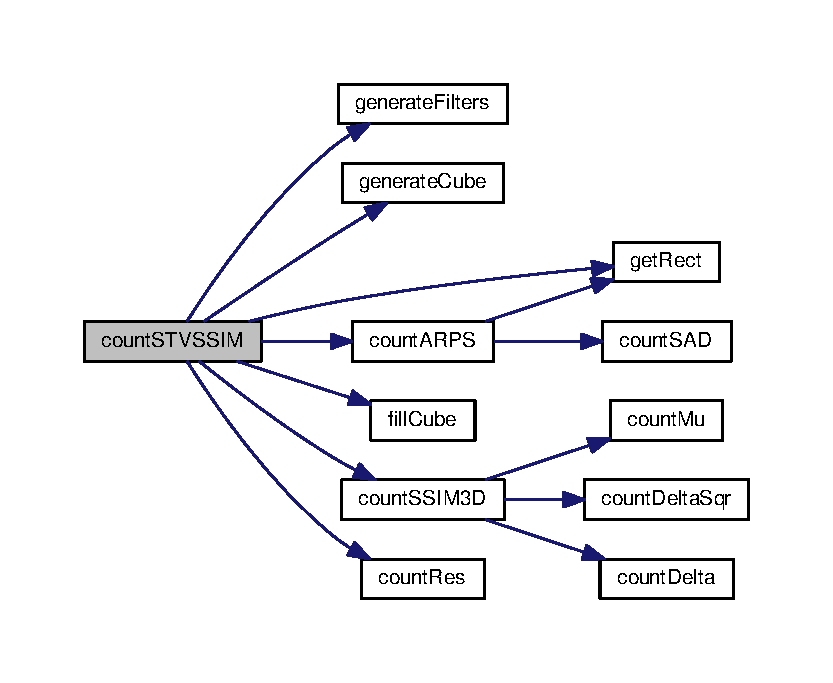
\includegraphics[width=350pt]{stvssim_8cpp_aa188224c32927a5f4e14c264724276ca_cgraph}
\end{center}
\end{figure}




Here is the caller graph for this function\-:
\nopagebreak
\begin{figure}[H]
\begin{center}
\leavevmode
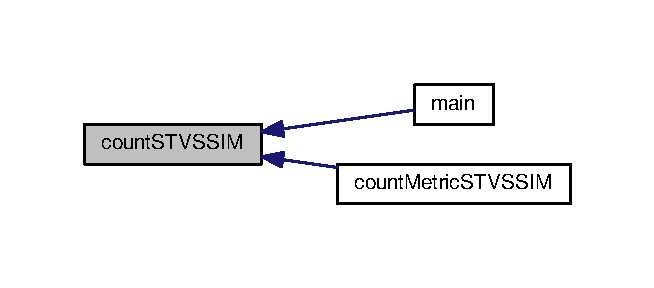
\includegraphics[width=314pt]{stvssim_8cpp_aa188224c32927a5f4e14c264724276ca_icgraph}
\end{center}
\end{figure}


\hypertarget{stvssim_8cpp_acafb1bf84ccd5750b7745d814c792560}{\index{stvssim.\-cpp@{stvssim.\-cpp}!fill\-Cube@{fill\-Cube}}
\index{fill\-Cube@{fill\-Cube}!stvssim.cpp@{stvssim.\-cpp}}
\subsubsection[{fill\-Cube}]{\setlength{\rightskip}{0pt plus 5cm}void fill\-Cube (
\begin{DoxyParamCaption}
\item[{unsigned char $\ast$$\ast$}]{datain, }
\item[{int}]{pos, }
\item[{unsigned char $\ast$$\ast$$\ast$}]{out, }
\item[{int}]{width}
\end{DoxyParamCaption}
)}}\label{stvssim_8cpp_acafb1bf84ccd5750b7745d814c792560}


Definition at line 261 of file stvssim.\-cpp.



Here is the caller graph for this function\-:
\nopagebreak
\begin{figure}[H]
\begin{center}
\leavevmode
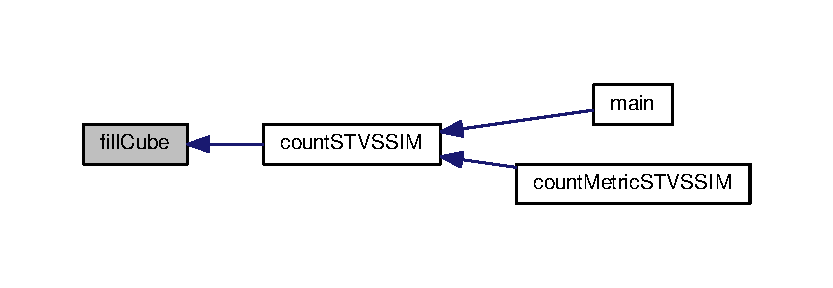
\includegraphics[width=350pt]{stvssim_8cpp_acafb1bf84ccd5750b7745d814c792560_icgraph}
\end{center}
\end{figure}


\hypertarget{stvssim_8cpp_aee5cce2c1f90ed16082c6f01eb8eb2ed}{\index{stvssim.\-cpp@{stvssim.\-cpp}!generate\-Cube@{generate\-Cube}}
\index{generate\-Cube@{generate\-Cube}!stvssim.cpp@{stvssim.\-cpp}}
\subsubsection[{generate\-Cube}]{\setlength{\rightskip}{0pt plus 5cm}unsigned char$\ast$$\ast$$\ast$ generate\-Cube (
\begin{DoxyParamCaption}
{}
\end{DoxyParamCaption}
)}}\label{stvssim_8cpp_aee5cce2c1f90ed16082c6f01eb8eb2ed}


Definition at line 248 of file stvssim.\-cpp.



Here is the caller graph for this function\-:
\nopagebreak
\begin{figure}[H]
\begin{center}
\leavevmode
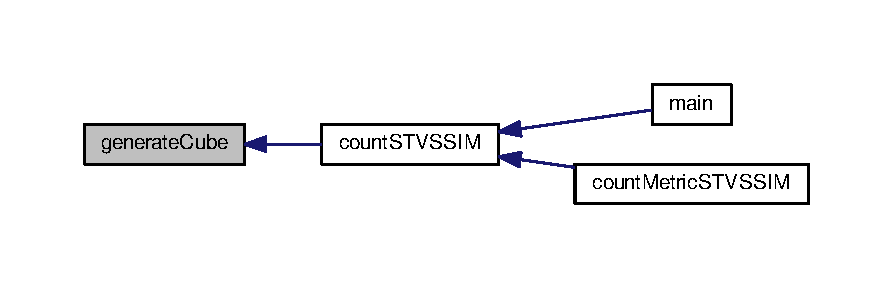
\includegraphics[width=350pt]{stvssim_8cpp_aee5cce2c1f90ed16082c6f01eb8eb2ed_icgraph}
\end{center}
\end{figure}


\hypertarget{stvssim_8cpp_a4094691210615420943d90d66fed89f0}{\index{stvssim.\-cpp@{stvssim.\-cpp}!generate\-Filters@{generate\-Filters}}
\index{generate\-Filters@{generate\-Filters}!stvssim.cpp@{stvssim.\-cpp}}
\subsubsection[{generate\-Filters}]{\setlength{\rightskip}{0pt plus 5cm}unsigned char$\ast$$\ast$$\ast$$\ast$ generate\-Filters (
\begin{DoxyParamCaption}
{}
\end{DoxyParamCaption}
)}}\label{stvssim_8cpp_a4094691210615420943d90d66fed89f0}


Definition at line 270 of file stvssim.\-cpp.



Here is the caller graph for this function\-:
\nopagebreak
\begin{figure}[H]
\begin{center}
\leavevmode
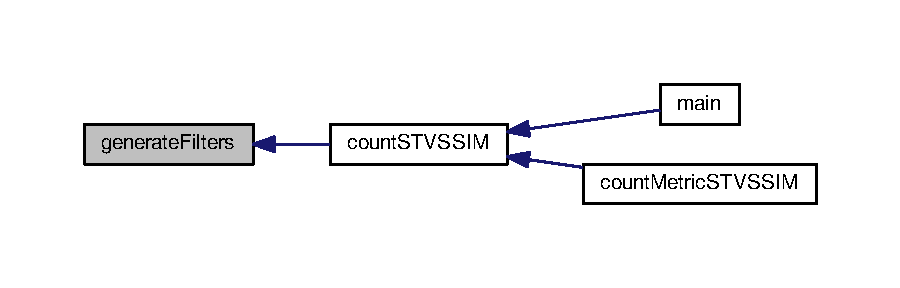
\includegraphics[width=350pt]{stvssim_8cpp_a4094691210615420943d90d66fed89f0_icgraph}
\end{center}
\end{figure}


\hypertarget{stvssim_8cpp_a23d24ef0b8f8b2069dfe95630f8e9181}{\index{stvssim.\-cpp@{stvssim.\-cpp}!shift\-Data@{shift\-Data}}
\index{shift\-Data@{shift\-Data}!stvssim.cpp@{stvssim.\-cpp}}
\subsubsection[{shift\-Data}]{\setlength{\rightskip}{0pt plus 5cm}void shift\-Data (
\begin{DoxyParamCaption}
\item[{unsigned char $\ast$$\ast$}]{data, }
\item[{int}]{size}
\end{DoxyParamCaption}
)}}\label{stvssim_8cpp_a23d24ef0b8f8b2069dfe95630f8e9181}


Definition at line 383 of file stvssim.\-cpp.



Here is the caller graph for this function\-:
\nopagebreak
\begin{figure}[H]
\begin{center}
\leavevmode
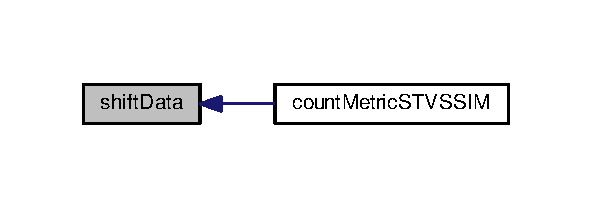
\includegraphics[width=284pt]{stvssim_8cpp_a23d24ef0b8f8b2069dfe95630f8e9181_icgraph}
\end{center}
\end{figure}



\hypertarget{stvssim_8h}{\section{src/stvssim.h File Reference}
\label{stvssim_8h}\index{src/stvssim.\-h@{src/stvssim.\-h}}
}
{\ttfamily \#include \char`\"{}main.\-h\char`\"{}}\\*
Include dependency graph for stvssim.\-h\-:
\nopagebreak
\begin{figure}[H]
\begin{center}
\leavevmode
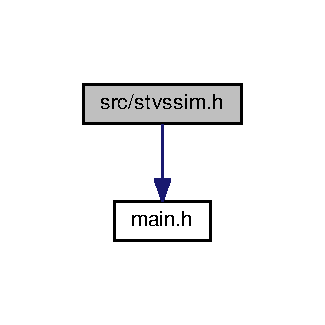
\includegraphics[width=156pt]{stvssim_8h__incl}
\end{center}
\end{figure}
This graph shows which files directly or indirectly include this file\-:
\nopagebreak
\begin{figure}[H]
\begin{center}
\leavevmode
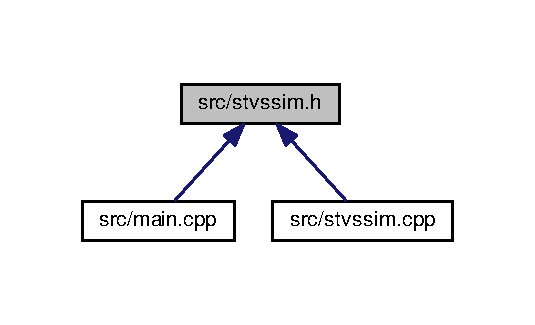
\includegraphics[width=257pt]{stvssim_8h__dep__incl}
\end{center}
\end{figure}
\subsection*{Classes}
\begin{DoxyCompactItemize}
\item 
struct \hyperlink{structvector}{vector}
\end{DoxyCompactItemize}
\subsection*{Macros}
\begin{DoxyCompactItemize}
\item 
\#define \hyperlink{stvssim_8h_a438c3ecdd60d36174c25c95baf4bc771}{R\-E\-C\-T\-\_\-\-S\-I\-Z\-E\-\_\-\-A\-R\-P\-S}~64
\item 
\#define \hyperlink{stvssim_8h_a58cf8bcd74e6572ffdb271b4d73b2eca}{R\-E\-C\-T\-\_\-\-S\-Q\-R\-T\-\_\-\-A\-R\-P\-S}~8
\item 
\#define \hyperlink{stvssim_8h_a6cf5fc8130ffce078802d200a2f415fc}{Z\-E\-R\-O\-\_\-\-M\-V\-M\-T}~12
\item 
\#define \hyperlink{stvssim_8h_a0decf52ffd72b5031b7fc6d09e98a3b1}{F\-R\-A\-M\-E\-\_\-\-C\-N\-T}~33
\item 
\#define \hyperlink{stvssim_8h_a2a7af63878a821bc2026c20b46b3e4e8}{R\-O\-O\-D\-\_\-\-S\-I\-Z\-E}~2
\item 
\#define \hyperlink{stvssim_8h_ac6a20f9818c203bfe2876cbd1e3bc8d5}{R\-E\-C\-T\-\_\-\-S\-Q\-R\-T\-\_\-3\-D}~11
\item 
\#define \hyperlink{stvssim_8h_a8f64a975405c2a6bc051f5799c2f28e4}{R\-E\-C\-T\-\_\-\-S\-I\-Z\-E\-\_\-3\-D}~11$\ast$11
\item 
\#define \hyperlink{stvssim_8h_a0c2b1b2d194b0322c812b4abbfc3872f}{F\-R\-A\-M\-E\-\_\-\-S\-K\-I\-P}~16
\item 
\#define \hyperlink{stvssim_8h_a9ec306f36d50c7375e74f0d1c55a3a67}{I\-N\-T\-\_\-\-M\-A\-X}~2147483647
\end{DoxyCompactItemize}
\subsection*{Functions}
\begin{DoxyCompactItemize}
\item 
double $\ast$$\ast$ \hyperlink{stvssim_8h_ac69b5b2265122a1b7775640b8feb43e6}{count\-Metric\-S\-T\-V\-S\-S\-I\-M} (F\-I\-L\-E $\ast$$\ast$streams, F\-I\-L\-E $\ast$ref, int files\-\_\-count, \hyperlink{structPictureData}{Picture\-Data} $\ast$frame, string type, double $\ast$$\ast$results, int $\ast$\&frames)
\item 
double \hyperlink{stvssim_8h_aa188224c32927a5f4e14c264724276ca}{count\-S\-T\-V\-S\-S\-I\-M} (unsigned char $\ast$$\ast$datain1, unsigned char $\ast$$\ast$datain2, int size, int width)
\item 
void \hyperlink{stvssim_8h_a23d24ef0b8f8b2069dfe95630f8e9181}{shift\-Data} (unsigned char $\ast$$\ast$data, int size)
\item 
\hyperlink{structvector}{vector} \hyperlink{stvssim_8h_a6aeaebf5f578aac2e9bdbf3151a571c5}{count\-A\-R\-P\-S} (unsigned char $\ast$block, unsigned char $\ast$frame\-Prev, int \hyperlink{png__decode_8cpp_a6150e0515f7202e2fb518f7206ed97dc}{x}, int \hyperlink{png__decode_8cpp_a0a2f84ed7838f07779ae24c5a9086d33}{y}, int width, int height, int T)
\item 
double \hyperlink{stvssim_8h_a32c2a80ad23848139ce03e3bf0d95b34}{count\-Delta} (unsigned char $\ast$$\ast$$\ast$filter, unsigned char $\ast$$\ast$$\ast$cube1, unsigned char $\ast$$\ast$$\ast$cube2, double mu\-X, double mu\-Y)
\item 
double \hyperlink{stvssim_8h_a1afca8ffefb48e73d9749f0902e6770e}{count\-Delta\-Sqr} (unsigned char $\ast$$\ast$$\ast$filter, unsigned char $\ast$$\ast$$\ast$cube, double mu)
\item 
double \hyperlink{stvssim_8h_ae81d1b26772887bce807b38ee044d8cf}{count\-Mu} (unsigned char $\ast$$\ast$$\ast$filter, unsigned char $\ast$$\ast$$\ast$cube)
\item 
double \hyperlink{stvssim_8h_ae40d916650014e6266ccbad2e3d08da9}{count\-S\-S\-I\-M3\-D} (unsigned char $\ast$$\ast$$\ast$filter, unsigned char $\ast$$\ast$$\ast$cube1, unsigned char $\ast$$\ast$$\ast$cube2)
\item 
unsigned char $\ast$$\ast$$\ast$ \hyperlink{stvssim_8h_aee5cce2c1f90ed16082c6f01eb8eb2ed}{generate\-Cube} ()
\item 
void \hyperlink{stvssim_8h_acafb1bf84ccd5750b7745d814c792560}{fill\-Cube} (unsigned char $\ast$$\ast$datain, int pos, unsigned char $\ast$$\ast$$\ast$out, int width)
\item 
unsigned char $\ast$$\ast$$\ast$$\ast$ \hyperlink{stvssim_8h_a4094691210615420943d90d66fed89f0}{generate\-Filters} ()
\item 
int \hyperlink{stvssim_8h_a0b34f8c2a0ca35e66931ea883c66397e}{count\-S\-A\-D} (unsigned char $\ast$rect1, unsigned char $\ast$rect2)
\end{DoxyCompactItemize}


\subsection{Macro Definition Documentation}
\hypertarget{stvssim_8h_a0decf52ffd72b5031b7fc6d09e98a3b1}{\index{stvssim.\-h@{stvssim.\-h}!F\-R\-A\-M\-E\-\_\-\-C\-N\-T@{F\-R\-A\-M\-E\-\_\-\-C\-N\-T}}
\index{F\-R\-A\-M\-E\-\_\-\-C\-N\-T@{F\-R\-A\-M\-E\-\_\-\-C\-N\-T}!stvssim.h@{stvssim.\-h}}
\subsubsection[{F\-R\-A\-M\-E\-\_\-\-C\-N\-T}]{\setlength{\rightskip}{0pt plus 5cm}\#define F\-R\-A\-M\-E\-\_\-\-C\-N\-T~33}}\label{stvssim_8h_a0decf52ffd72b5031b7fc6d09e98a3b1}


Definition at line 7 of file stvssim.\-h.

\hypertarget{stvssim_8h_a0c2b1b2d194b0322c812b4abbfc3872f}{\index{stvssim.\-h@{stvssim.\-h}!F\-R\-A\-M\-E\-\_\-\-S\-K\-I\-P@{F\-R\-A\-M\-E\-\_\-\-S\-K\-I\-P}}
\index{F\-R\-A\-M\-E\-\_\-\-S\-K\-I\-P@{F\-R\-A\-M\-E\-\_\-\-S\-K\-I\-P}!stvssim.h@{stvssim.\-h}}
\subsubsection[{F\-R\-A\-M\-E\-\_\-\-S\-K\-I\-P}]{\setlength{\rightskip}{0pt plus 5cm}\#define F\-R\-A\-M\-E\-\_\-\-S\-K\-I\-P~16}}\label{stvssim_8h_a0c2b1b2d194b0322c812b4abbfc3872f}


Definition at line 11 of file stvssim.\-h.

\hypertarget{stvssim_8h_a9ec306f36d50c7375e74f0d1c55a3a67}{\index{stvssim.\-h@{stvssim.\-h}!I\-N\-T\-\_\-\-M\-A\-X@{I\-N\-T\-\_\-\-M\-A\-X}}
\index{I\-N\-T\-\_\-\-M\-A\-X@{I\-N\-T\-\_\-\-M\-A\-X}!stvssim.h@{stvssim.\-h}}
\subsubsection[{I\-N\-T\-\_\-\-M\-A\-X}]{\setlength{\rightskip}{0pt plus 5cm}\#define I\-N\-T\-\_\-\-M\-A\-X~2147483647}}\label{stvssim_8h_a9ec306f36d50c7375e74f0d1c55a3a67}


Definition at line 12 of file stvssim.\-h.

\hypertarget{stvssim_8h_a8f64a975405c2a6bc051f5799c2f28e4}{\index{stvssim.\-h@{stvssim.\-h}!R\-E\-C\-T\-\_\-\-S\-I\-Z\-E\-\_\-3\-D@{R\-E\-C\-T\-\_\-\-S\-I\-Z\-E\-\_\-3\-D}}
\index{R\-E\-C\-T\-\_\-\-S\-I\-Z\-E\-\_\-3\-D@{R\-E\-C\-T\-\_\-\-S\-I\-Z\-E\-\_\-3\-D}!stvssim.h@{stvssim.\-h}}
\subsubsection[{R\-E\-C\-T\-\_\-\-S\-I\-Z\-E\-\_\-3\-D}]{\setlength{\rightskip}{0pt plus 5cm}\#define R\-E\-C\-T\-\_\-\-S\-I\-Z\-E\-\_\-3\-D~11$\ast$11}}\label{stvssim_8h_a8f64a975405c2a6bc051f5799c2f28e4}


Definition at line 10 of file stvssim.\-h.

\hypertarget{stvssim_8h_a438c3ecdd60d36174c25c95baf4bc771}{\index{stvssim.\-h@{stvssim.\-h}!R\-E\-C\-T\-\_\-\-S\-I\-Z\-E\-\_\-\-A\-R\-P\-S@{R\-E\-C\-T\-\_\-\-S\-I\-Z\-E\-\_\-\-A\-R\-P\-S}}
\index{R\-E\-C\-T\-\_\-\-S\-I\-Z\-E\-\_\-\-A\-R\-P\-S@{R\-E\-C\-T\-\_\-\-S\-I\-Z\-E\-\_\-\-A\-R\-P\-S}!stvssim.h@{stvssim.\-h}}
\subsubsection[{R\-E\-C\-T\-\_\-\-S\-I\-Z\-E\-\_\-\-A\-R\-P\-S}]{\setlength{\rightskip}{0pt plus 5cm}\#define R\-E\-C\-T\-\_\-\-S\-I\-Z\-E\-\_\-\-A\-R\-P\-S~64}}\label{stvssim_8h_a438c3ecdd60d36174c25c95baf4bc771}


Definition at line 4 of file stvssim.\-h.

\hypertarget{stvssim_8h_ac6a20f9818c203bfe2876cbd1e3bc8d5}{\index{stvssim.\-h@{stvssim.\-h}!R\-E\-C\-T\-\_\-\-S\-Q\-R\-T\-\_\-3\-D@{R\-E\-C\-T\-\_\-\-S\-Q\-R\-T\-\_\-3\-D}}
\index{R\-E\-C\-T\-\_\-\-S\-Q\-R\-T\-\_\-3\-D@{R\-E\-C\-T\-\_\-\-S\-Q\-R\-T\-\_\-3\-D}!stvssim.h@{stvssim.\-h}}
\subsubsection[{R\-E\-C\-T\-\_\-\-S\-Q\-R\-T\-\_\-3\-D}]{\setlength{\rightskip}{0pt plus 5cm}\#define R\-E\-C\-T\-\_\-\-S\-Q\-R\-T\-\_\-3\-D~11}}\label{stvssim_8h_ac6a20f9818c203bfe2876cbd1e3bc8d5}


Definition at line 9 of file stvssim.\-h.

\hypertarget{stvssim_8h_a58cf8bcd74e6572ffdb271b4d73b2eca}{\index{stvssim.\-h@{stvssim.\-h}!R\-E\-C\-T\-\_\-\-S\-Q\-R\-T\-\_\-\-A\-R\-P\-S@{R\-E\-C\-T\-\_\-\-S\-Q\-R\-T\-\_\-\-A\-R\-P\-S}}
\index{R\-E\-C\-T\-\_\-\-S\-Q\-R\-T\-\_\-\-A\-R\-P\-S@{R\-E\-C\-T\-\_\-\-S\-Q\-R\-T\-\_\-\-A\-R\-P\-S}!stvssim.h@{stvssim.\-h}}
\subsubsection[{R\-E\-C\-T\-\_\-\-S\-Q\-R\-T\-\_\-\-A\-R\-P\-S}]{\setlength{\rightskip}{0pt plus 5cm}\#define R\-E\-C\-T\-\_\-\-S\-Q\-R\-T\-\_\-\-A\-R\-P\-S~8}}\label{stvssim_8h_a58cf8bcd74e6572ffdb271b4d73b2eca}


Definition at line 5 of file stvssim.\-h.

\hypertarget{stvssim_8h_a2a7af63878a821bc2026c20b46b3e4e8}{\index{stvssim.\-h@{stvssim.\-h}!R\-O\-O\-D\-\_\-\-S\-I\-Z\-E@{R\-O\-O\-D\-\_\-\-S\-I\-Z\-E}}
\index{R\-O\-O\-D\-\_\-\-S\-I\-Z\-E@{R\-O\-O\-D\-\_\-\-S\-I\-Z\-E}!stvssim.h@{stvssim.\-h}}
\subsubsection[{R\-O\-O\-D\-\_\-\-S\-I\-Z\-E}]{\setlength{\rightskip}{0pt plus 5cm}\#define R\-O\-O\-D\-\_\-\-S\-I\-Z\-E~2}}\label{stvssim_8h_a2a7af63878a821bc2026c20b46b3e4e8}


Definition at line 8 of file stvssim.\-h.

\hypertarget{stvssim_8h_a6cf5fc8130ffce078802d200a2f415fc}{\index{stvssim.\-h@{stvssim.\-h}!Z\-E\-R\-O\-\_\-\-M\-V\-M\-T@{Z\-E\-R\-O\-\_\-\-M\-V\-M\-T}}
\index{Z\-E\-R\-O\-\_\-\-M\-V\-M\-T@{Z\-E\-R\-O\-\_\-\-M\-V\-M\-T}!stvssim.h@{stvssim.\-h}}
\subsubsection[{Z\-E\-R\-O\-\_\-\-M\-V\-M\-T}]{\setlength{\rightskip}{0pt plus 5cm}\#define Z\-E\-R\-O\-\_\-\-M\-V\-M\-T~12}}\label{stvssim_8h_a6cf5fc8130ffce078802d200a2f415fc}


Definition at line 6 of file stvssim.\-h.



\subsection{Function Documentation}
\hypertarget{stvssim_8h_a6aeaebf5f578aac2e9bdbf3151a571c5}{\index{stvssim.\-h@{stvssim.\-h}!count\-A\-R\-P\-S@{count\-A\-R\-P\-S}}
\index{count\-A\-R\-P\-S@{count\-A\-R\-P\-S}!stvssim.h@{stvssim.\-h}}
\subsubsection[{count\-A\-R\-P\-S}]{\setlength{\rightskip}{0pt plus 5cm}{\bf vector} count\-A\-R\-P\-S (
\begin{DoxyParamCaption}
\item[{unsigned char $\ast$}]{block, }
\item[{unsigned char $\ast$}]{frame\-Prev, }
\item[{int}]{x, }
\item[{int}]{y, }
\item[{int}]{width, }
\item[{int}]{height, }
\item[{int}]{T}
\end{DoxyParamCaption}
)}}\label{stvssim_8h_a6aeaebf5f578aac2e9bdbf3151a571c5}


Definition at line 316 of file stvssim.\-cpp.



Here is the call graph for this function\-:
\nopagebreak
\begin{figure}[H]
\begin{center}
\leavevmode
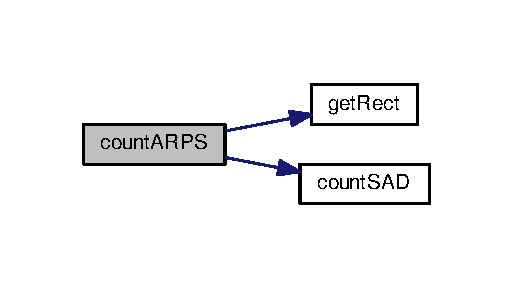
\includegraphics[width=246pt]{stvssim_8h_a6aeaebf5f578aac2e9bdbf3151a571c5_cgraph}
\end{center}
\end{figure}




Here is the caller graph for this function\-:
\nopagebreak
\begin{figure}[H]
\begin{center}
\leavevmode
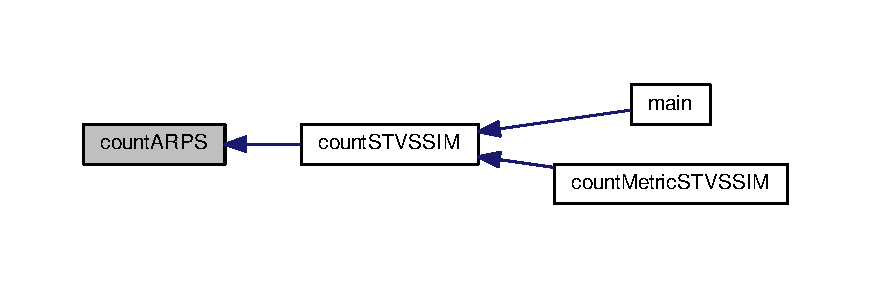
\includegraphics[width=350pt]{stvssim_8h_a6aeaebf5f578aac2e9bdbf3151a571c5_icgraph}
\end{center}
\end{figure}


\hypertarget{stvssim_8h_a32c2a80ad23848139ce03e3bf0d95b34}{\index{stvssim.\-h@{stvssim.\-h}!count\-Delta@{count\-Delta}}
\index{count\-Delta@{count\-Delta}!stvssim.h@{stvssim.\-h}}
\subsubsection[{count\-Delta}]{\setlength{\rightskip}{0pt plus 5cm}double count\-Delta (
\begin{DoxyParamCaption}
\item[{unsigned char $\ast$$\ast$$\ast$}]{filter, }
\item[{unsigned char $\ast$$\ast$$\ast$}]{cube1, }
\item[{unsigned char $\ast$$\ast$$\ast$}]{cube2, }
\item[{double}]{mu\-X, }
\item[{double}]{mu\-Y}
\end{DoxyParamCaption}
)}}\label{stvssim_8h_a32c2a80ad23848139ce03e3bf0d95b34}


Definition at line 235 of file stvssim.\-cpp.



Here is the caller graph for this function\-:
\nopagebreak
\begin{figure}[H]
\begin{center}
\leavevmode
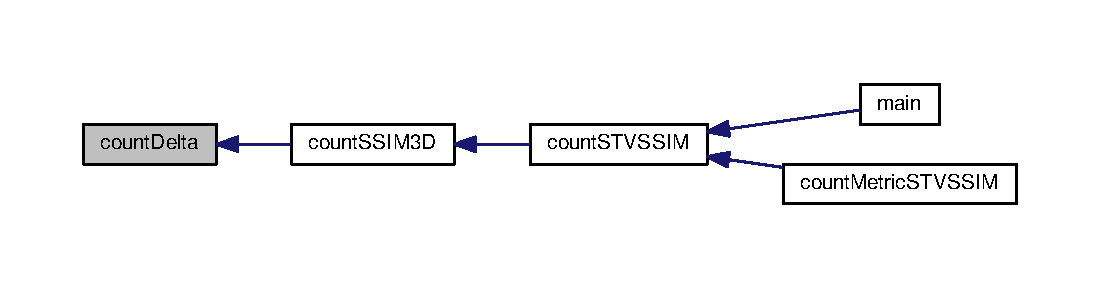
\includegraphics[width=350pt]{stvssim_8h_a32c2a80ad23848139ce03e3bf0d95b34_icgraph}
\end{center}
\end{figure}


\hypertarget{stvssim_8h_a1afca8ffefb48e73d9749f0902e6770e}{\index{stvssim.\-h@{stvssim.\-h}!count\-Delta\-Sqr@{count\-Delta\-Sqr}}
\index{count\-Delta\-Sqr@{count\-Delta\-Sqr}!stvssim.h@{stvssim.\-h}}
\subsubsection[{count\-Delta\-Sqr}]{\setlength{\rightskip}{0pt plus 5cm}double count\-Delta\-Sqr (
\begin{DoxyParamCaption}
\item[{unsigned char $\ast$$\ast$$\ast$}]{filter, }
\item[{unsigned char $\ast$$\ast$$\ast$}]{cube, }
\item[{double}]{mu}
\end{DoxyParamCaption}
)}}\label{stvssim_8h_a1afca8ffefb48e73d9749f0902e6770e}


Definition at line 222 of file stvssim.\-cpp.



Here is the caller graph for this function\-:
\nopagebreak
\begin{figure}[H]
\begin{center}
\leavevmode
\includegraphics[width=350pt]{stvssim_8h_a1afca8ffefb48e73d9749f0902e6770e_icgraph}
\end{center}
\end{figure}


\hypertarget{stvssim_8h_ac69b5b2265122a1b7775640b8feb43e6}{\index{stvssim.\-h@{stvssim.\-h}!count\-Metric\-S\-T\-V\-S\-S\-I\-M@{count\-Metric\-S\-T\-V\-S\-S\-I\-M}}
\index{count\-Metric\-S\-T\-V\-S\-S\-I\-M@{count\-Metric\-S\-T\-V\-S\-S\-I\-M}!stvssim.h@{stvssim.\-h}}
\subsubsection[{count\-Metric\-S\-T\-V\-S\-S\-I\-M}]{\setlength{\rightskip}{0pt plus 5cm}double$\ast$$\ast$ count\-Metric\-S\-T\-V\-S\-S\-I\-M (
\begin{DoxyParamCaption}
\item[{F\-I\-L\-E $\ast$$\ast$}]{streams, }
\item[{F\-I\-L\-E $\ast$}]{ref, }
\item[{int}]{files\-\_\-count, }
\item[{{\bf Picture\-Data} $\ast$}]{frame, }
\item[{string}]{type, }
\item[{double $\ast$$\ast$}]{results, }
\item[{int $\ast$\&}]{frames}
\end{DoxyParamCaption}
)}}\label{stvssim_8h_ac69b5b2265122a1b7775640b8feb43e6}


Definition at line 16 of file stvssim.\-cpp.



Here is the call graph for this function\-:
\nopagebreak
\begin{figure}[H]
\begin{center}
\leavevmode
\includegraphics[width=350pt]{stvssim_8h_ac69b5b2265122a1b7775640b8feb43e6_cgraph}
\end{center}
\end{figure}


\hypertarget{stvssim_8h_ae81d1b26772887bce807b38ee044d8cf}{\index{stvssim.\-h@{stvssim.\-h}!count\-Mu@{count\-Mu}}
\index{count\-Mu@{count\-Mu}!stvssim.h@{stvssim.\-h}}
\subsubsection[{count\-Mu}]{\setlength{\rightskip}{0pt plus 5cm}double count\-Mu (
\begin{DoxyParamCaption}
\item[{unsigned char $\ast$$\ast$$\ast$}]{filter, }
\item[{unsigned char $\ast$$\ast$$\ast$}]{cube}
\end{DoxyParamCaption}
)}}\label{stvssim_8h_ae81d1b26772887bce807b38ee044d8cf}


Definition at line 208 of file stvssim.\-cpp.



Here is the caller graph for this function\-:
\nopagebreak
\begin{figure}[H]
\begin{center}
\leavevmode
\includegraphics[width=350pt]{stvssim_8h_ae81d1b26772887bce807b38ee044d8cf_icgraph}
\end{center}
\end{figure}


\hypertarget{stvssim_8h_a0b34f8c2a0ca35e66931ea883c66397e}{\index{stvssim.\-h@{stvssim.\-h}!count\-S\-A\-D@{count\-S\-A\-D}}
\index{count\-S\-A\-D@{count\-S\-A\-D}!stvssim.h@{stvssim.\-h}}
\subsubsection[{count\-S\-A\-D}]{\setlength{\rightskip}{0pt plus 5cm}int count\-S\-A\-D (
\begin{DoxyParamCaption}
\item[{unsigned char $\ast$}]{rect1, }
\item[{unsigned char $\ast$}]{rect2}
\end{DoxyParamCaption}
)}}\label{stvssim_8h_a0b34f8c2a0ca35e66931ea883c66397e}


Definition at line 390 of file stvssim.\-cpp.



Here is the caller graph for this function\-:
\nopagebreak
\begin{figure}[H]
\begin{center}
\leavevmode
\includegraphics[width=350pt]{stvssim_8h_a0b34f8c2a0ca35e66931ea883c66397e_icgraph}
\end{center}
\end{figure}


\hypertarget{stvssim_8h_ae40d916650014e6266ccbad2e3d08da9}{\index{stvssim.\-h@{stvssim.\-h}!count\-S\-S\-I\-M3\-D@{count\-S\-S\-I\-M3\-D}}
\index{count\-S\-S\-I\-M3\-D@{count\-S\-S\-I\-M3\-D}!stvssim.h@{stvssim.\-h}}
\subsubsection[{count\-S\-S\-I\-M3\-D}]{\setlength{\rightskip}{0pt plus 5cm}double count\-S\-S\-I\-M3\-D (
\begin{DoxyParamCaption}
\item[{unsigned char $\ast$$\ast$$\ast$}]{filter, }
\item[{unsigned char $\ast$$\ast$$\ast$}]{cube1, }
\item[{unsigned char $\ast$$\ast$$\ast$}]{cube2}
\end{DoxyParamCaption}
)}}\label{stvssim_8h_ae40d916650014e6266ccbad2e3d08da9}


Definition at line 196 of file stvssim.\-cpp.



Here is the call graph for this function\-:
\nopagebreak
\begin{figure}[H]
\begin{center}
\leavevmode
\includegraphics[width=274pt]{stvssim_8h_ae40d916650014e6266ccbad2e3d08da9_cgraph}
\end{center}
\end{figure}




Here is the caller graph for this function\-:
\nopagebreak
\begin{figure}[H]
\begin{center}
\leavevmode
\includegraphics[width=350pt]{stvssim_8h_ae40d916650014e6266ccbad2e3d08da9_icgraph}
\end{center}
\end{figure}


\hypertarget{stvssim_8h_aa188224c32927a5f4e14c264724276ca}{\index{stvssim.\-h@{stvssim.\-h}!count\-S\-T\-V\-S\-S\-I\-M@{count\-S\-T\-V\-S\-S\-I\-M}}
\index{count\-S\-T\-V\-S\-S\-I\-M@{count\-S\-T\-V\-S\-S\-I\-M}!stvssim.h@{stvssim.\-h}}
\subsubsection[{count\-S\-T\-V\-S\-S\-I\-M}]{\setlength{\rightskip}{0pt plus 5cm}double count\-S\-T\-V\-S\-S\-I\-M (
\begin{DoxyParamCaption}
\item[{unsigned char $\ast$$\ast$}]{datain1, }
\item[{unsigned char $\ast$$\ast$}]{datain2, }
\item[{int}]{size, }
\item[{int}]{width}
\end{DoxyParamCaption}
)}}\label{stvssim_8h_aa188224c32927a5f4e14c264724276ca}


Definition at line 81 of file stvssim.\-cpp.



Here is the call graph for this function\-:
\nopagebreak
\begin{figure}[H]
\begin{center}
\leavevmode
\includegraphics[width=350pt]{stvssim_8h_aa188224c32927a5f4e14c264724276ca_cgraph}
\end{center}
\end{figure}




Here is the caller graph for this function\-:
\nopagebreak
\begin{figure}[H]
\begin{center}
\leavevmode
\includegraphics[width=314pt]{stvssim_8h_aa188224c32927a5f4e14c264724276ca_icgraph}
\end{center}
\end{figure}


\hypertarget{stvssim_8h_acafb1bf84ccd5750b7745d814c792560}{\index{stvssim.\-h@{stvssim.\-h}!fill\-Cube@{fill\-Cube}}
\index{fill\-Cube@{fill\-Cube}!stvssim.h@{stvssim.\-h}}
\subsubsection[{fill\-Cube}]{\setlength{\rightskip}{0pt plus 5cm}void fill\-Cube (
\begin{DoxyParamCaption}
\item[{unsigned char $\ast$$\ast$}]{datain, }
\item[{int}]{pos, }
\item[{unsigned char $\ast$$\ast$$\ast$}]{out, }
\item[{int}]{width}
\end{DoxyParamCaption}
)}}\label{stvssim_8h_acafb1bf84ccd5750b7745d814c792560}


Definition at line 261 of file stvssim.\-cpp.



Here is the caller graph for this function\-:
\nopagebreak
\begin{figure}[H]
\begin{center}
\leavevmode
\includegraphics[width=350pt]{stvssim_8h_acafb1bf84ccd5750b7745d814c792560_icgraph}
\end{center}
\end{figure}


\hypertarget{stvssim_8h_aee5cce2c1f90ed16082c6f01eb8eb2ed}{\index{stvssim.\-h@{stvssim.\-h}!generate\-Cube@{generate\-Cube}}
\index{generate\-Cube@{generate\-Cube}!stvssim.h@{stvssim.\-h}}
\subsubsection[{generate\-Cube}]{\setlength{\rightskip}{0pt plus 5cm}unsigned char$\ast$$\ast$$\ast$ generate\-Cube (
\begin{DoxyParamCaption}
{}
\end{DoxyParamCaption}
)}}\label{stvssim_8h_aee5cce2c1f90ed16082c6f01eb8eb2ed}


Definition at line 248 of file stvssim.\-cpp.



Here is the caller graph for this function\-:
\nopagebreak
\begin{figure}[H]
\begin{center}
\leavevmode
\includegraphics[width=350pt]{stvssim_8h_aee5cce2c1f90ed16082c6f01eb8eb2ed_icgraph}
\end{center}
\end{figure}


\hypertarget{stvssim_8h_a4094691210615420943d90d66fed89f0}{\index{stvssim.\-h@{stvssim.\-h}!generate\-Filters@{generate\-Filters}}
\index{generate\-Filters@{generate\-Filters}!stvssim.h@{stvssim.\-h}}
\subsubsection[{generate\-Filters}]{\setlength{\rightskip}{0pt plus 5cm}unsigned char$\ast$$\ast$$\ast$$\ast$ generate\-Filters (
\begin{DoxyParamCaption}
{}
\end{DoxyParamCaption}
)}}\label{stvssim_8h_a4094691210615420943d90d66fed89f0}


Definition at line 270 of file stvssim.\-cpp.



Here is the caller graph for this function\-:
\nopagebreak
\begin{figure}[H]
\begin{center}
\leavevmode
\includegraphics[width=350pt]{stvssim_8h_a4094691210615420943d90d66fed89f0_icgraph}
\end{center}
\end{figure}


\hypertarget{stvssim_8h_a23d24ef0b8f8b2069dfe95630f8e9181}{\index{stvssim.\-h@{stvssim.\-h}!shift\-Data@{shift\-Data}}
\index{shift\-Data@{shift\-Data}!stvssim.h@{stvssim.\-h}}
\subsubsection[{shift\-Data}]{\setlength{\rightskip}{0pt plus 5cm}void shift\-Data (
\begin{DoxyParamCaption}
\item[{unsigned char $\ast$$\ast$}]{data, }
\item[{int}]{size}
\end{DoxyParamCaption}
)}}\label{stvssim_8h_a23d24ef0b8f8b2069dfe95630f8e9181}


Definition at line 73 of file main.\-cpp.



Here is the caller graph for this function\-:
\nopagebreak
\begin{figure}[H]
\begin{center}
\leavevmode
\includegraphics[width=284pt]{stvssim_8h_a23d24ef0b8f8b2069dfe95630f8e9181_icgraph}
\end{center}
\end{figure}



%--- End generated contents ---

% Index
\newpage
\phantomsection
\addcontentsline{toc}{chapter}{Index}
\printindex

\end{document}
